% informe_tecnico.tex
% Compilar con pdflatex (requiere babel[spanish], inputenc[utf8], y tablas)
\documentclass[12pt,letterpaper]{article}
\usepackage[utf8]{inputenc}
\usepackage[spanish]{babel}
\usepackage{geometry}
\geometry{top=2.5cm, bottom=2.5cm, left=2.5cm, right=2.5cm}
\usepackage{graphicx}
\usepackage{subcaption}
\usepackage{array}
\usepackage{multirow}
\usepackage{booktabs}
\usepackage{longtable}
\usepackage{adjustbox}
\usepackage{xcolor}
\usepackage{amssymb}
\usepackage{hyperref}
\hypersetup{
	colorlinks=true,
	linkcolor=blue,
	urlcolor=blue,
}
\usepackage{listings}
\usepackage{caption}
\usepackage{float}

\lstset{
	basicstyle=\ttfamily\small,
	breaklines=true,
	frame=single,
	language=bash,
	inputencoding=utf8,
	extendedchars=true,
	literate={á}{{\'a}}1 {é}{{\'e}}1 {í}{{\'i}}1 {ó}{{\'o}}1 {ú}{{\'u}}1
	{Á}{{\'A}}1 {É}{{\'E}}1 {Í}{{\'I}}1 {Ó}{{\'O}}1 {Ú}{{\'U}}1
	{ñ}{{\~n}}1 {Ñ}{{\~N}}1 {ü}{{\"u}}1 {Ü}{{\"U}}1,
}

% Configuración de código
\lstset{
	basicstyle=\ttfamily\small,
	breaklines=true,
	frame=single,
	language=bash,
}

\title{Sistema web para el autorreporte de Eventos Supuestamente Atribuibles a la Vacunación o Inmunización (ESAVI) en el Instituto Finlay de Vacunas (IFV)}
\author{Jabel Resendiz Aguirre}
\date{\today}

\begin{document}

\begin{titlepage}
	\centering

	\begin{minipage}{0.45\textwidth}
		\centering
		
\includegraphics[width=0.55\textwidth]{Graphics/uhlogo.pdf}
	\end{minipage}
	\hfill
	\begin{minipage}{0.45\textwidth}
		\centering
		
\includegraphics[width=0.95\textwidth]{Graphics/logo.jpg}
	\end{minipage}

	\vspace{1cm}

	{\Large\textbf{Universidad de La Habana}\\
	\textbf{Facultad de Matemática y Computación}\par}

	\vspace{1cm}

	{\LARGE\bfseries Informe Técnico de Software\par}

	\vspace{0.8cm}

	{\Large\bfseries Sistema web para el autorreporte de Eventos Supuestamente Atribuibles a la Vacunación o Inmunización (ESAVI) en el Instituto Finlay de Vacunas (IFV)\par}

	\vspace{1.2cm}

	\begin{center}
	\begin{tabular}{p{3.8cm} p{9cm}}
		\textbf{Proyecto:} & Sistema web para el autorreporte de ESAVI en el IFV \\
		\textbf{Organización:} & Instituto Finlay de Vacunas (IFV) \\
		\textbf{Autor:} & Jabel Resendiz Aguirre \\
		\textbf{Facultad:} & Facultad de Matemática y Computación \\
		\textbf{Fecha:} & \today \\
		\textbf{Clasificación:} & Público \\
	\end{tabular}
	\end{center}

	\vfill

\end{titlepage}

\newpage
\tableofcontents
\newpage
	

\section*{Control de Versiones}
\addcontentsline{toc}{section}{Control de Versiones}

\begin{table}[H]
\centering
\caption{Historial de cambios del documento}
\label{tab:historial}
\begin{tabular}{|l|l|l|l|}
\hline
\textbf{Versión} & \textbf{Fecha} & \textbf{Autor} & \textbf{Descripción del cambio} \\ \hline
1.0.0 & 15/08/2026 & Jabel Resendiz & Versión inicial del informe técnico \\ \hline
\end{tabular}
\end{table}



	\newpage
	\section{Resumen Ejecutivo}

El proyecto consiste en un sistema web orientado al autorreporte de eventos supuestamente atribuibles a la vacunación o inmunización (ESAVI) para el Instituto Finlay de Vacunas. La solución permite a los reporteros registrar incidentes relacionados con la vacunación, hacer seguimiento del estado de cada notificación y brindar herramientas de revisión a profesionales médicos, responsables de sección y administradores. La arquitectura combina un frontend en React y TypeScript con un backend en ASP.NET Core 8, con persistencia en MySQL, mensajería con RabbitMQ y despliegue mediante contenedores Docker.

El sistema se encuentra en una etapa de desarrollo y validación funcional, con componentes operativos para autenticación, gestión de reportes, dashboards, catálogos de vacunas y síntomas, asignación médica, manejo de centros de vacunación y lotes. La solución ofrece un flujo de trabajo que va desde la captura pública del reporte hasta la revisión y administración interna, con control de acceso por roles y mecanismos de seguridad como JWT, refresh tokens y limitación de peticiones.

Los beneficios esperados del sistema son la reducción de los tiempos de registro y seguimiento de los ESAVI, la estandarización de la información recopilada, la trazabilidad de cada caso y la mejora en la toma de decisiones por parte de las áreas técnicas y médicas del instituto.

\section{Alcance y Objetivos}

\subsection{Propósito del sistema}

El sistema responde a la necesidad de contar con un canal digital seguro y formalizado para el reporte de eventos adversos asociados a vacunas. Su propósito es centralizar la información de los casos reportados, facilitar su revisión por personal médico y permitir a la organización mantener trazabilidad y control sobre los incidentes notificados.

La plataforma también busca reducir la dependencia de procesos manuales, mejorar la calidad de la información y ofrecer una vista operativa para la administración de reportes, usuarios, catálogos y asignaciones internas.

\subsection{Alcance del proyecto}

\textbf{Alcance incluido:}
\begin{itemize}
\item Registro público de reportes de ESAVI desde el frontend.
\item Seguimiento del estado de cada reporte mediante número de notificación.
\item Autenticación de usuarios con roles de administrador, responsable de sección, revisor médico y usuario estándar.
\item Dashboards y consultas para monitoreo de reportes y métricas generales.
\item Gestión de catálogos de vacunas, síntomas, manufacturas, centros de vacunación y lotes.
\item Asignación y reasignación de reportes para revisión médica.
\item Detección y resolución de reportes duplicados.
\end{itemize}

\textbf{Alcance excluido:}
\begin{itemize}
\item Aplicación móvil nativa.
\item Funcionamiento en modo offline.
\item Integración directa con sistemas externos de farmacovigilancia o plataformas regulatorias.
\item Soporte multilenguaje o adaptación completa a múltiples regiones.
\end{itemize}

\textbf{Supuestos:}
\begin{itemize}
\item El entorno de desarrollo cuenta con Docker, MySQL y RabbitMQ disponibles.
\item Los usuarios acceden desde navegadores modernos con conexión a internet.
\item Los datos de salud reportados requieren tratamiento confidencial y restringido a usuarios autorizados.
\end{itemize}

\textbf{Restricciones:}
\begin{itemize}
\item La implementación actual está enfocada a un entorno interno y no contempla despliegue distribuido a gran escala.
\item El repositorio visible no incluye una suite automatizada de pruebas completa.
\item La configuración de variables de entorno y secretos depende del operario de despliegue.
\end{itemize}
	











	\section{Requisitos del Sistema}

\subsection{Requisitos funcionales}

Los requisitos funcionales definen las capacidades que el sistema debe ofrecer para la captura, gestión, seguimiento y análisis de los reportes de ESAVI, abarcando los diferentes perfiles de usuario identificados en el diagrama de casos de uso.

\begin{table}[H]
\centering
\caption{Requisitos funcionales}
\label{tab:rf}
\begin{tabular}{|l|p{8cm}|l|}
\hline
\textbf{ID} & \textbf{Requisito} & \textbf{Prioridad} \\[2pt] \hline
RF-01 & Registrar reportes ESAVI mediante formulario web estructurado. & Crítica \\ \hline
RF-02 & Generar código único de notificación por reporte exitoso. & Crítica \\ \hline
RF-03 & Validar campos obligatorios antes del envío del reporte. & Crítica \\ \hline
RF-04 & Almacenar reportes en base de datos centralizada. & Crítica \\ \hline
RF-05 & Gestionar estado del reporte (enviado, revisión, aprobado, rechazado, cerrado). & Crítica \\ \hline
RF-06 & Ofrecer consulta con búsqueda, filtrado y ordenación según rol. & Crítica \\ \hline
RF-07 & Autenticar usuarios y administrar roles para acceso a funcionalidades. & Crítica \\ \hline
RF-08 & Generar estadísticas y visualizaciones gráficas de eventos y rendimiento. & Alta \\ \hline
RF-09 & Exportar información a PDF y Excel para análisis institucionales. & Alta \\ \hline
RF-10 & Enviar notificaciones automáticas según eventos del flujo y rol del usuario. & Alta \\ \hline
RF-11 & Detectar duplicados automáticamente y permitir veredicto manual. & Alta \\ \hline
RF-12 & Reasignar reportes cuya fecha límite de evaluación haya sido superada. & Alta \\ \hline
\end{tabular}
\end{table}

\subsection{Requisitos no funcionales}

Los requisitos no funcionales definen las condiciones de calidad bajo las cuales debe operar la solución. 
En la Tabla \ref{tab:rnf} se resumen los atributos considerados más relevantes.
	

\begin{table}[H]
\centering
\caption{Requisitos no funcionales}
\label{tab:rnf}
\begin{tabular}{|l|p{8cm}|l|}
\hline
\textbf{ID} & \textbf{Requisito} & \textbf{Categoría} \\
\hline
RNF-01 & Interfaz intuitiva con elementos estructurados (listas, botones, casillas), minimizando texto libre. & Usabilidad \\ \hline
RNF-02 & Cumplir pautas WCAG 2.1 nivel AA para personas con discapacidades. & Accesibilidad \\ \hline
RNF-03 & Adaptarse a escritorio, tabletas y dispositivos móviles. & Diseño responsivo \\ \hline
RNF-04 & Compatible con Chrome, Firefox, Edge y Safari. & Compatibilidad \\ \hline
RNF-05 & Procesar envío de reporte en menos de 3 segundos (sin latencia de red externa). & Rendimiento \\ \hline
RNF-06 & Diseño modular con separación clara de componentes para facilitar mantenimiento y escalabilidad. & Mantenibilidad \\ \hline
RNF-07 & Garantizar confidencialidad, integridad y disponibilidad mediante autenticación, control de acceso y cifrado. & Seguridad \\ \hline
RNF-08 & Registrar acciones de usuarios (creación, modificación, actualización) para auditoría y trazabilidad. & Auditoría \\ \hline
\end{tabular}
\end{table}


\subsection{Requisitos de entorno}

El proyecto fue diseñado para operar en tres niveles de entorno, garantizando la consistencia mediante contenerización con Docker y facilitando la migración progresiva hacia la infraestructura institucional del IFV.

\begin{table}[H]
\centering
\caption{Requisitos de entorno}
\label{tab:entorno}
\begin{tabular}{|l|p{3.5cm}|p{3.5cm}|p{3.5cm}|}
\hline
\textbf{Componente} & \textbf{Desarrollo} & \textbf{Demostración} & \textbf{Producción futura} \\[2pt] \hline
Frontend & Vite/React local & Vercel & Servidor institucional con HTTPS \\ \hline
Backend & API .NET 8 local & Railway & Servidor dedicado del IFV \\ \hline
Base de datos & MySQL 8 en contenedor & MySQL en Railway & MySQL administrado internamente \\ \hline
Mensajería & RabbitMQ local & RabbitMQ en Railway & RabbitMQ o servicio interno \\ \hline
Red & Localhost y puertos expuestos & Red interna o VPN & HTTPS con reglas de firewall \\ \hline
\end{tabular}
\end{table}

	


	\section{Contexto y Casos de Uso}

\subsection{Descripción del sistema}

El sistema se denomina plataforma web para el autorreporte de ESAVI del Instituto Finlay de Vacunas. Es una aplicación web de arquitectura cliente-servidor, con frontend SPA en React y backend REST en ASP.NET Core. La solución está pensada para operación interna y de uso institucional, con acceso a través de navegadores modernos en entornos web.

\subsection{Identificación de los actores}

De acuerdo con el modelado funcional, el sistema cuenta con cinco actores principales que interactúan con la plataforma de gestión de vacunación y ESAVI:

\begin{itemize}
\item \textbf{Usuario Autenticado:} Actor abstracto que representa la base de permisos comunes. De él heredan todos los roles que requieren autenticación en el sistema.
\item \textbf{Jefe de Vacunación Municipal:} Hereda de Usuario. Responsable de la supervisión local, encargado de la gestión del personal médico y la distribución de la carga de trabajo.
\item \textbf{Médico Evaluador:} Hereda de Usuario. Profesional sanitario encargado del análisis clínico de los eventos reportados.
\item \textbf{Administrador:} Hereda de Usuario. Representa al personal del IFV que supervisa el proceso y monitorea el comportamiento de la asignación y revisión de reportes en cada territorio.
\item \textbf{Reportante:} Actor independiente sin autenticación. Representa a la persona que notifica un evento adverso al sistema.
\end{itemize}

\subsection{Diagrama de casos de uso}

La figura \ref{fig:diagrama_casos_uso} recoge los casos de uso del sistema. El diagrama organiza las funcionalidades según el actor que las ejecuta y refleja las relaciones de extensión entre casos de uso.

\begin{figure}[H]
\centering
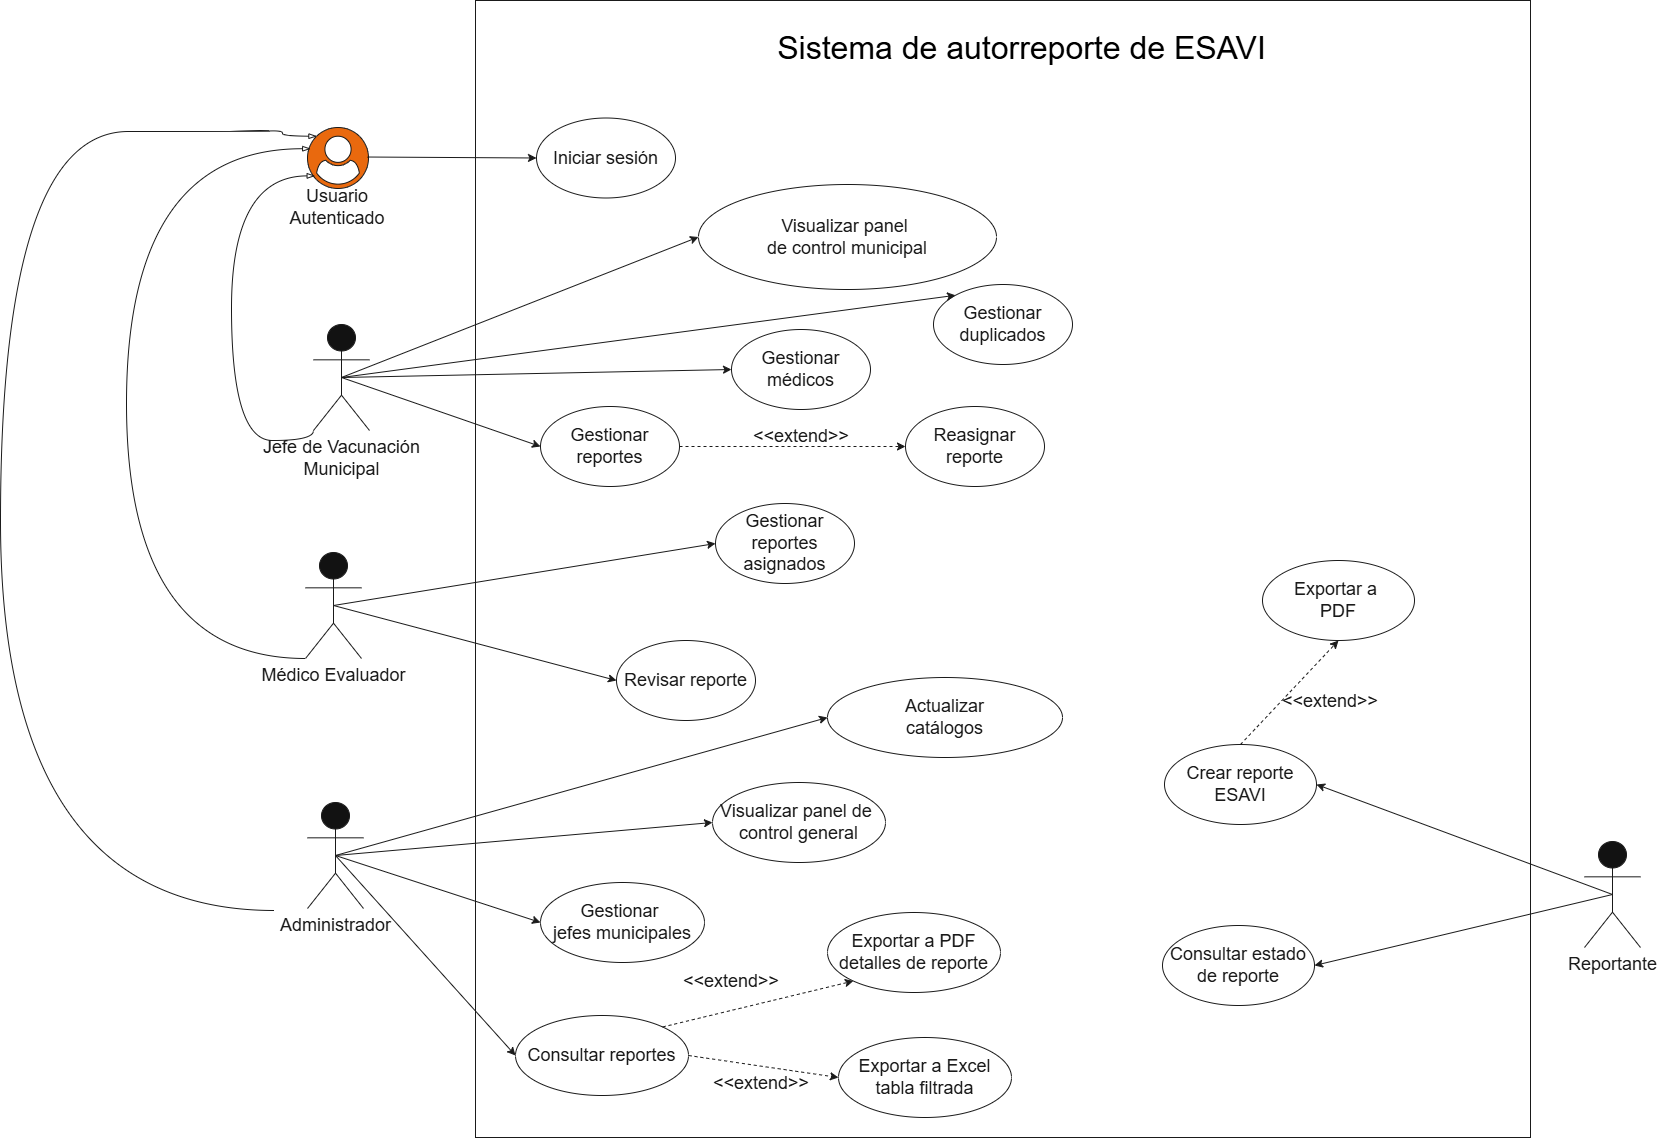
\includegraphics[scale=0.2]{Graphics/casos_uso.drawio.png}
\caption[Diagrama de casos de uso]{Diagrama de casos de usos.}
\label{fig:diagrama_casos_uso}
\end{figure}

\subsection{Especificación de casos de uso principales}

A continuación se describe la lógica de negocio asociada a cada interacción:

\begin{itemize}
\item \textbf{Iniciar sesión:} Caso de uso base que permite el acceso controlado a la plataforma según las credenciales del usuario (correo electrónico y contraseña). Este caso de uso es común a los roles de jefe de vacunación municipal, médico evaluador y administrador, quienes heredan esta funcionalidad del actor usuario autenticado. El reportante, al ser un actor independiente sin autenticación, no tiene acceso a esta funcionalidad.

\item \textbf{Gestión de reportes (Reportante):}
\begin{itemize}
\item \textbf{Crear reporte ESAVI:} Permite el ingreso de un nuevo reporte mediante un formulario estructurado que captura información del sujeto vacunado, datos médicos previos, vacunación, eventos adversos y datos del reportante. Al completar el envío, el sistema genera un número de notificación único, envía un mensaje al jefe de vacunación del municipio correspondiente sobre el nuevo reporte. Este caso de uso posee una relación de tipo \textit{extend} hacia \textbf{Exportar a PDF}, lo que indica que el usuario puede, opcionalmente, generar un comprobante documental tras completar el registro.
\item \textbf{Consultar estado de reporte:} Permite al reportante verificar el estado de sus envíos previos ingresando el número de notificación.
\end{itemize}

\item \textbf{Supervisión Municipal (Jefe de Vacunación):}
\begin{itemize}
\item \textbf{Gestionar reportes:} Permite al jefe de vacunación visualizar los reportes de su municipio en una tabla filtrable por gravedad, vacuna, estado del reporte y ordenable por fecha. Desde esta vista, puede seleccionar un reporte y asignarlo a un médico evaluador disponible. Al asignar, el sistema registra la fecha límite de evaluación según la prioridad del reporte (ver RN-08). De manera opcional (\textit{extend}), puede \textbf{Reasignar reporte}: cuando una asignación supera su plazo de evaluación sin que el médico la haya completado, el jefe reasigna el reporte a otro médico. La asignación anterior pasa a estado \texttt{cancelado} y crea una nueva con una fecha límite actualizada.
\item \textbf{Gestionar duplicados:} Permite al jefe de vacunación acceder a una cola de revisión que lista los posibles duplicados detectados por el sistema (ver RN-09). Al seleccionar un caso, el sistema muestra una vista comparativa lado a lado entre el reporte original y la copia. El jefe emite un veredicto manual mediante una de estas acciones: \textbf{Confirmar duplicado} (descarta la copia del flujo y registra la resolución) o \textbf{Separar como caso nuevo} (libera la copia al flujo normal y registra la resolución). Este control de calidad es previo a la asignación y garantiza la integridad de los datos antes de que un caso llegue a un médico evaluador.
\item \textbf{Visualizar panel de control municipal:} Ofrece un panel con indicadores agregados del municipio: reportes totales, pendientes, en revisión y completados; tiempos promedio de revisión y de asignación; promedio de asignaciones por reporte; distribución de reportes por rango de tiempo de completitud; distribución porcentual de estados por médico; carga activa de trabajo por médico; y los elementos más reportados: vacunas, síntomas y distribución por gravedad, junto con una línea de tiempo de reportes. Estos indicadores permiten al jefe identificar qué médicos están más ocupados, cuáles responden con mayor rapidez y tomar decisiones sobre la distribución de la carga de trabajo.
\item \textbf{Gestionar médicos:} Permite al jefe de vacunación dar de alta a los médicos evaluadores bajo su jurisdicción. El jefe ingresa el correo electrónico y el número de registro profesional del médico. El sistema envía un enlace de activación al correo del médico, quien completa su registro estableciendo su contraseña y confirmando su número de registro profesional. Este mecanismo garantiza que solo el médico legítimo active su cuenta y que la contraseña no sea conocida por terceros.
\end{itemize}

\item \textbf{Gestión Clínica (Médico Evaluador):}
\begin{itemize}
\item \textbf{Gestionar reportes asignados:} Vista principal donde el médico visualiza los reportes que le han sido asignados por el jefe de vacunación de su municipio. Cada reporte muestra el número de notificación, la fecha de creación y la gravedad. La tabla permite filtrar y ordenar por antigüedad, gravedad u otros criterios para priorizar la carga de trabajo.
\item \textbf{Revisar reporte:} El médico accede al detalle del reporte, analiza la información clínica del sujeto vacunado, los datos de vacunación y los eventos adversos descritos. A partir de esta información, determina la causalidad del evento, emite un dictamen y completa la revisión. La regla RN-08 establece el plazo máximo para completar esta evaluación según la prioridad del reporte. Al finalizar, el sistema notifica al jefe de vacunación sobre la conclusión de la evaluación.
\end{itemize}

\item \textbf{Administración y Configuración (Administrador):}
\begin{itemize}
\item \textbf{Actualizar catálogos:} Permite al administrador mantener actualizados los catálogos del sistema: vacunas, síntomas, lotes y centros de vacunación.
\item \textbf{Gestionar jefes municipales:} Permite al administrador dar de alta a los jefes de vacunación municipal. El sistema envía un enlace de activación al correo electrónico del jefe, quien completa su registro estableciendo su contraseña.
\item \textbf{Consultar reportes:} Permite al administrador visualizar una tabla con todos los reportes del sistema, filtrable por vacuna, gravedad, estado del reporte y provincia. Cada fila muestra información preliminar del reporte —edad, sexo, provincia, vacunas, eventos adversos, gravedad, estado y médico asignado— y permite acceder al detalle completo del reporte. De manera opcional (\textit{extend}), puede \textbf{Exportar a Excel} la tabla filtrada y \textbf{Exportar a PDF} el detalle de un reporte.
\item \textbf{Visualizar panel de control:} Ofrece un panel con indicadores agregados y gráficos interactivos. Incluye tendencias de reportes por estado, distribución geográfica por provincias, reportes por gravedad y por causalidad, indicadores de rendimiento —número de médicos activos, promedio de reportes por médico, tiempos de revisión y de asignación— y los elementos más reportados: vacunas, lotes por vacuna y síntomas.
\end{itemize}
\end{itemize}

\subsection{Reglas de negocio}

Las reglas de negocio definen las restricciones y políticas que rigen la operación del sistema:

\begin{itemize}
\item \textbf{RN-01. Alcance territorial del jefe de vacunación:} Un jefe de vacunación solo puede gestionar reportes y asignar médicos evaluadores exclusivamente dentro del municipio al que está adscrito.

\item \textbf{RN-02. Asignación exclusiva:} Un reporte solo puede estar asignado a un único médico evaluador a la vez. Cualquier nueva asignación —ya sea inicial o por reasignación— cancela la anterior.

\item \textbf{RN-03. Unicidad de vacuna por fecha:} El sistema no permite que un reportante seleccione la misma vacuna del catálogo más de una vez en la misma fecha para un mismo sujeto vacunado.

\item \textbf{RN-04. Consistencia cronológica:} Las fechas registradas en un reporte deben respetar las siguientes restricciones. La fecha de nacimiento del sujeto y del reportante antecede a todas las fechas de vacunación y de inicio de eventos adversos. Cada fecha de inicio de evento adverso es posterior o igual a todas las fechas de vacunación. Si un evento adverso registra fecha de fin, esta debe ser posterior o igual a su fecha de inicio. Cualquier fecha de fallecimiento debe ser posterior o igual al inicio de los eventos adversos y anterior o igual a la fecha de reporte y a la fecha actual.

\item \textbf{RN-05. Integridad del reporte:} Todo reporte debe contener al menos un evento adverso y una vacuna asociada para ser enviado.

\item \textbf{RN-06. Gravedad derivada:} El sistema clasifica automáticamente un evento adverso como serio si el reportante marcó al menos uno de los criterios de gravedad registrados en el reporte. En caso contrario, lo clasifica como no serio. El usuario no interviene directamente sobre este campo.

\item \textbf{RN-07. Priorización de reportes por nivel de riesgo:} El sistema clasifica cada reporte según el evento adverso más grave que contenga. La prioridad responde al siguiente criterio:
\begin{itemize}
\item \textbf{Prioridad alta:} el evento es serio (resultó en muerte, hospitalización, visita al doctor o a emergencias, discapacidad permanente o anomalía congénita).
\item \textbf{Prioridad media:} el evento no es serio pero la intensidad del síntoma es severa, o el sujeto vacunado continúa sin recuperarse o presenta secuelas.
\item \textbf{Prioridad baja:} el evento no cumple ninguna de las restricciones anteriores (evento no serio, sujeto recuperado, en recuperación, desconocido, intensidad breve).
\end{itemize}

\item \textbf{RN-08. Plazo de evaluación según prioridad:} Los reportes de prioridad alta deben evaluarse en un máximo de 24 horas; los de prioridad media, en un máximo de 5 días; los de prioridad baja, en un máximo de 7 días. Cada asignación registra su fecha límite al momento de crearse. Superado el plazo, el sistema notifica al médico evaluador y al jefe de vacunación correspondiente, pero no modifica automáticamente el estado de la asignación. Para determinar si una revisión cumplió el plazo, el sistema compara la fecha en que finalizó con la fecha límite registrada.

\item \textbf{RN-09. Detección de posibles duplicados:} Al registrarse un nuevo reporte, el sistema verificará si ya existe en la base de datos otro reporte que comparta el mismo identificador del sujeto vacunado, la misma fecha de vacunación y la misma vacuna. En caso de coincidencia, el sistema insertará automáticamente un registro en la tabla de control de duplicados, estableciendo: el reporte preexistente como \texttt{original}, el reporte recién creado como \texttt{copia}, y el estado inicial como \texttt{posible\_duplicado}. Un reporte que figure como \texttt{copia} en dicha tabla con estado \texttt{posible\_duplicado} no podrá ser asignado a ningún evaluador ni avanzar en el flujo de farmacovigilancia hasta que un usuario especializado emita un veredicto manual que confirme o descarte la duplicidad.
\end{itemize}










\section{Arquitectura del Sistema}

\subsection{Vista arquitectónica general}

La arquitectura del sistema sigue un patrón por capas, con separación entre frontend, API, lógica de aplicación, dominio e infraestructura. El frontend actúa como cliente SPA que consume servicios REST del backend. El backend expone controladores REST, utiliza servicios de aplicación y un repositorio/unidad de trabajo para encapsular el acceso a datos. La infraestructura gestiona MySQL, RabbitMQ y los procesos de inicialización y logging.

La figura \ref{fig:arquitectura} ilustra la organización completa del sistema bajo el modelo de arquitectura limpia, mostrando cómo cada capa se relaciona con las adyacentes y cómo las dependencias apuntan siempre hacia el núcleo del dominio.

\begin{figure}[H]
\centering
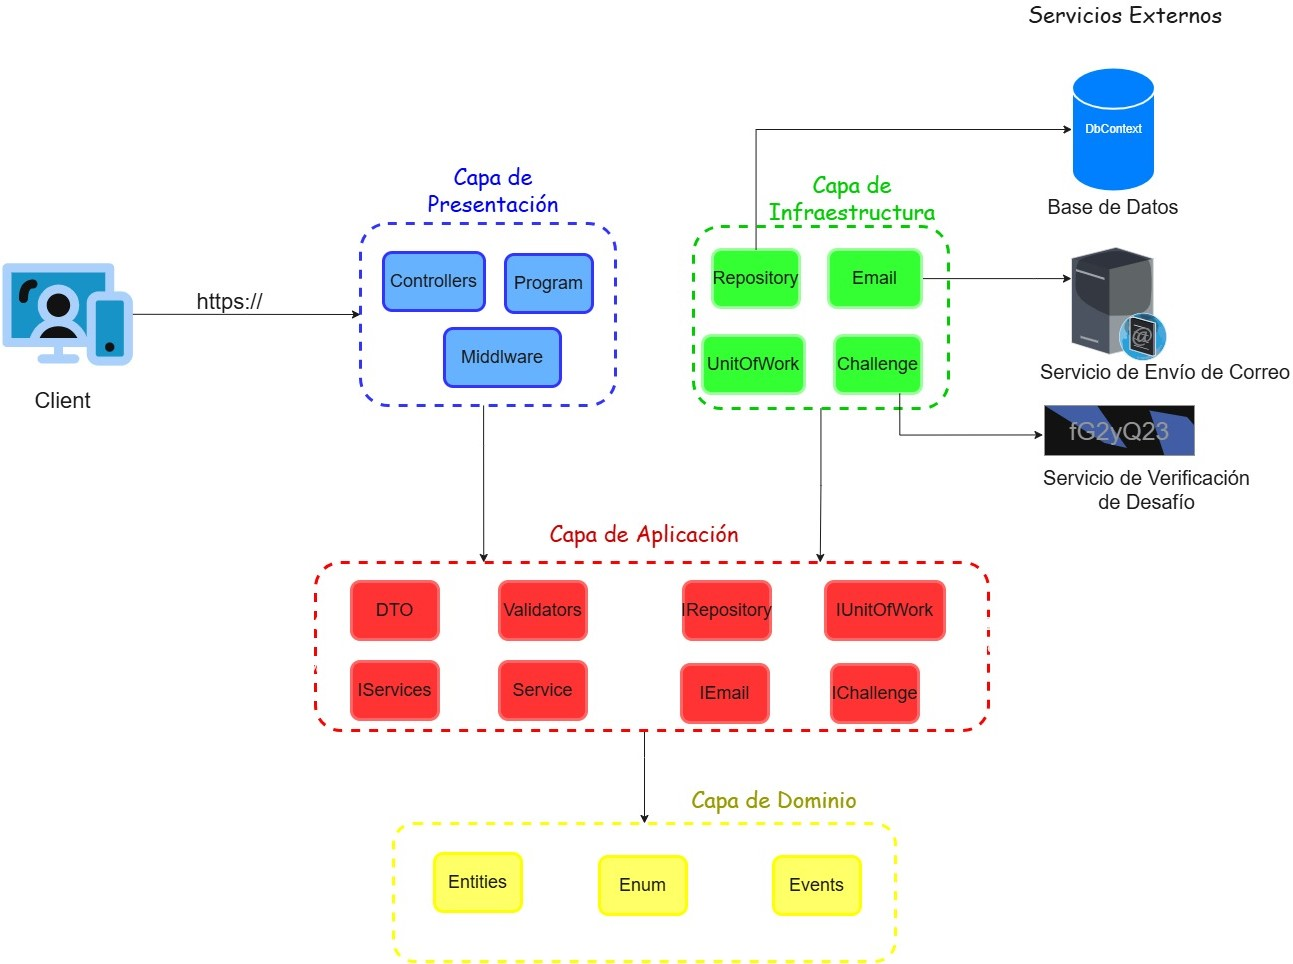
\includegraphics[scale=0.55]{Graphics/arquitectura.jpg}
\caption[Vista arquitectónica general del sistema]{Vista arquitectónica general del sistema bajo el modelo de arquitectura limpia. Fuente: elaboración propia.}
\label{fig:arquitectura}
\end{figure}

La arquitectura se organiza en cuatro niveles concéntricos que reflejan la regla de dependencia de la arquitectura limpia: las capas externas dependen de las internas, pero nunca al revés. En el centro se encuentra la capa de dominio, que contiene las entidades de negocio y las reglas fundamentales del sistema. Alrededor de esta, la capa de aplicación orquesta los casos de uso y define las interfaces que la infraestructura debe implementar. La capa de infraestructura proporciona las implementaciones concretas de persistencia, mensajería y servicios externos. Finalmente, la capa de presentación expone la funcionalidad a través de una API REST que es consumida por el frontend.

El flujo de comunicación entre componentes sigue un orden descendente que respeta esta organización:

\begin{itemize}
\item El \textbf{frontend} (React + TypeScript) realiza peticiones HTTP/JSON al backend mediante Axios.
\item La \textbf{API REST} (ASP.NET Core 8) recibe estas peticiones y las traduce en invocaciones a los casos de uso de la capa de aplicación.
\item La \textbf{capa de aplicación} aplica las validaciones necesarias, orquesta la lógica de negocio y utiliza los repositorios definidos mediante interfaces para acceder a los datos.
\item La \textbf{capa de infraestructura} implementa estas interfaces proporcionando acceso a MySQL mediante EF Core, gestiona la mensajería a través de RabbitMQ y registra las operaciones mediante Serilog.
\item El \textbf{dominio} contiene las entidades y objetos de valor que modelan el negocio, sin ningún tipo de dependencia externa.
\end{itemize}

\subsection{Componentes principales}

La tabla \ref{tab:componentes} desglosa los componentes fundamentales que conforman el sistema, especificando su responsabilidad, la tecnología empleada y sus dependencias dentro de la arquitectura.

\begin{table}[H]
\centering
\caption{Componentes principales}
\label{tab:componentes}
\begin{tabular}{|l|p{7cm}|p{3cm}|p{3cm}|}
\hline
\textbf{Componente} & \textbf{Responsabilidad} & \textbf{Tecnología} & \textbf{Dependencias} \\ \hline
Frontend SPA & Renderiza vistas, formularios, dashboards y navegación por roles & React + TypeScript + Vite & Axios, React Router, MUI/Radix  \\ \hline
API REST & Expone endpoints para autenticación, reportes, catálogos y dashboards & ASP.NET Core 8 & Application, Infrastructure \\ \hline
Capa de aplicación & Valida reglas de negocio y orquesta casos de uso & Services + DTOs + Validators & Domain, Infrastructure \\ \hline
Persistencia & Almacena entidades de reportes, usuarios, vacunas y revisiones & EF Core + MySQL & Unit of Work, Repositories \\ \hline
Mensajería & Soporta flujos asíncronos y procesamiento de eventos & RabbitMQ & Consumers, BackgroundServices \\ \hline
\end{tabular}
\end{table}

Cada componente ha sido diseñado con responsabilidades claramente delimitadas para facilitar el mantenimiento y la evolución del sistema. La separación entre la capa de aplicación y la de infraestructura permite que los cambios tecnológicos —como migrar de MySQL a PostgreSQL o sustituir RabbitMQ por Azure Service Bus— no afecten la lógica de negocio central, siempre que se respeten los contratos definidos en las interfaces.

\subsection{Patrones de diseño aplicados}

Para garantizar la calidad estructural del sistema y facilitar su evolución, se han aplicado varios patrones de diseño ampliamente reconocidos. La tabla \ref{tab:patrones} resume los patrones implementados, su categoría y su aplicación concreta en el sistema ESAVI.

\begin{table}[H]
\centering
\caption{Patrones aplicados}
\label{tab:patrones}
\begin{tabular}{|l|p{2.6cm}|p{8.4cm}|}
\hline
\textbf{Patrón} & \textbf{Categoría} & \textbf{Aplicación en el sistema} \\ \hline
Repositorio & Persistencia & Abstrae el acceso a datos mediante interfaces, permitiendo al dominio obtener y almacenar objetos sin conocer los detalles de persistencia. Declarado en aplicación e implementado en infraestructura con EF Core. \\ \hline
Unit of Work & Persistencia & Agrupa operaciones sobre repositorios y las persiste de forma atómica, garantizando que los cambios de una transacción se confirmen o descarten como una sola unidad . \\ \hline
Inyección de dependencias & Creacional & Servicios y repositorios registrados en el contenedor de ASP.NET Core, permitiendo que cada capa trabaje con interfaces sin conocer los detalles de construcción de sus dependencias . \\ \hline
Mapper (DTO) & Estructural & Convierte objetos entre capas mediante DTOs, transportando solo los datos necesarios en cada límite. Mantiene el dominio encapsulado y permite evolución independiente de capas. \\ \hline
Separación CQS & Arquitectónico & Separa operaciones en comandos (modifican estado) y consultas (retornan datos), facilitando pruebas unitarias y evolución independiente de cada interfaz. \\ \hline
\end{tabular}
\end{table}

La implementación del patrón Repositorio junto con Unit of Work garantiza que las operaciones de base de datos se realicen de forma atómica, manteniendo la consistencia de los datos incluso en operaciones que involucran múltiples entidades. La Inyección de dependencias actúa como mecanismo de desacoplamiento entre capas, permitiendo sustituir implementaciones sin afectar al núcleo del sistema. Por su parte, el Mapper mediante DTOs asegura que el dominio permanezca encapsulado y que cada capa pueda evolucionar de forma independiente, mientras que la Separación CQS facilita las pruebas unitarias y permite que cada interfaz evolucione según sus necesidades. Esta organización por capas, junto con los patrones descritos, conforma una arquitectura mantenible y flexible ante futuros cambios regulatorios o tecnológicos.

\subsection{Comunicación entre componentes}

La comunicación entre los componentes del sistema se divide en dos modalidades: síncrona y asíncrona. La comunicación síncrona entre frontend y backend se realiza mediante peticiones REST sobre HTTP/JSON, utilizando Axios en el cliente y controladores ASP.NET Core en el servidor. La comunicación asíncrona se apoya en RabbitMQ para procesos de mensajería o integración de eventos cuando el sistema requiera desacoplar tareas.

El flujo de comunicación sigue el siguiente patrón:
\begin{itemize}
\item El frontend envía peticiones HTTP al backend a través de la API REST.
\item Los controladores de la API traducen estas peticiones en invocaciones a los casos de uso de la capa de aplicación.
\item Los casos de uso coordinan las operaciones necesarias, interactuando con el dominio y utilizando los repositorios para acceder a los datos.
\item Cuando se requiere procesamiento asíncrono —como el envío de notificaciones por correo electrónico o la generación de reportes en segundo plano—, la capa de aplicación publica mensajes en RabbitMQ.
\item Los consumidores de RabbitMQ procesan estos mensajes de forma independiente, sin bloquear el flujo principal de la aplicación.
\end{itemize}










	\section{Tecnologías y Dependencias}
	
	\subsection{Stack tecnológico}
	
	\begin{table}[H]
		\centering
		\caption{Stack tecnológico completo}
		\label{tab:stack}
		\begin{tabular}{|l|l|l|l|}
			\hline
			\textbf{Capa} & \textbf{Tecnología} & \textbf{Versión} & \textbf{Licencia} \\ \hline
			Frontend & React + TypeScript + Vite & 18.3.1 / 7.x & MIT \\ \hline
			Backend & ASP.NET Core 8 + C\# & .NET 8.0 & MIT \\ \hline
			Base de datos & MySQL & 8.0 & GPL / comercial \\ \hline
			Mensajería & RabbitMQ + MassTransit & 3.x / 8.3.0 & MPL-2.0 / Apache-2.0 \\ \hline
			Contenedores & Docker Compose & 3.8 / Docker 24.x & Apache-2.0 \\ \hline
		\end{tabular}
	\end{table}
	
	\subsection{Dependencias externas}
	
	\begin{table}[H]
		\centering
		\caption{Dependencias principales del proyecto}
		\label{tab:deps}
		\begin{tabular}{|p{7cm}|l|p{5cm}|p{2cm}|}
			\hline
			\textbf{Paquete} & \textbf{Versión} & \textbf{Propósito} & \textbf{Licencia} \\ \hline
			\texttt{react} & \verb|18.3.1| & Biblioteca principal del frontend & MIT \\ \hline
			\texttt{@mui/material} & \verb|7.3.5| & Componentes y diseño visual & MIT \\ \hline
			\texttt{react-router-dom} & \verb|^7.17.0| & Enrutamiento de vistas & MIT \\ \hline
			\texttt{Microsoft.AspNetCore.} \newline \texttt{Authentication.JwtBearer} & \verb|8.0.0| & Seguridad con JWT & MIT \\ \hline
			
			\texttt{Pomelo.EntityFrameworkCore.MySql} & \verb|8.0.0| & Provider de MySQL para EF Core & MIT \\ \hline
			\texttt{MassTransit.RabbitMQ} & \verb|8.3.0| & Integración con RabbitMQ & Apache-2.0 \\ \hline
			\texttt{MailKit} & \verb|4.15.1| & Envío de correos electrónicos & MIT \\ \hline
			\texttt{QuestPDF} & \verb|2026.6.0| & Generación de documentos PDF & MIT \\ \hline
		\end{tabular}
	\end{table}
	
	\subsection{Justificación técnica}
	
	La solución se diseñó con un enfoque basado en una arquitectura parcialmente desacoplada, combinando un frontend moderno con un backend empresarial. 
	
	Para la capa de servicios, se eligió \textbf{ASP.NET Core 8} por su alta eficiencia de recursos y ecosistema integrado, que supera a Spring Boot en consumo de memoria y a NestJS en rendimiento en tareas intensivas. 
	Para la persistencia, se optó por \textbf{MySQL} dentro del paradigma relacional, ofreciendo un equilibrio entre integración con Entity Framework Core, licencia de código abierto y despliegue multiplataforma frente a SQL Server y PostgreSQL. En mensajería, \textbf{RabbitMQ} permite desacoplar procesos asíncronos como notificaciones y alertas sin bloquear la experiencia del usuario. Para la interfaz, \textbf{React con TypeScript y Vite} proporciona el equilibrio entre eficiencia, flexibilidad y mantenibilidad necesario para interfaces con formularios dinámicos como los requeridos por el sistema de farmacovigilancia.






	\section{Estructura del Código Fuente}
	
	\subsection{Organización de directorios}
	
	La estructura del proyecto refleja una separación clara entre frontend, backend y capas de negocio. La organización actual del repositorio es la siguiente:
	
	\begin{verbatim}
		esavi-report/
		  backend/
		    Finlay.PharmaVigilance.API/
		      Controllers/
		      Middleware/
		      Common/
		      Program.cs
		    Finlay.PharmaVigilance.Application/
		      Services/
		      DTOs/
		      Validators/
		      IServices/
		      IRepository/
		    Finlay.PharmaVigilance.Domain/
		      Entities/
		      Enum/
		      ValueObjects/
		      Events/
		    Finlay.PharmaVigilance.Infrastructure/
		      Repository/
		      Authentication/
		      Consumers/
		      EventBus/
		      Pdf/
		      Contact/
		      Migrations/
		      FinlayDbContext.cs
		  frontend/
		    src/
		      app/
		      assets/
		      services/
		      styles/
		      types/
		    package.json
		    vite.config.ts
		    Dockerfile
	\end{verbatim}
	
	Esta distribución responde a una arquitectura por capas: la API expone endpoints, la capa de aplicación implementa casos de uso, el dominio encapsula entidades y reglas de negocio, y la infraestructura gestiona acceso a datos, autenticación, mensajería y generación de documentos.
	
	\subsection{Convenciones de código}
	
	\begin{itemize}
		\item En el backend, las clases y servicios se nombran en PascalCase; las variables y métodos siguen camelCase; las interfaces se identifican con prefijo \texttt{I} (por ejemplo, \texttt{IService}, \texttt{IRepository}).
		\item El dominio modela entidades, enums, value objects y eventos, manteniendo la lógica de negocio separada de la infraestructura.
		\item La infraestructura centraliza persistencia, autenticación JWT, mensajería RabbitMQ, envío de correos y generación de PDF.
		\item El frontend se organiza en módulos bajo \texttt{src/app}, servicios bajo \texttt{src/services} y recursos compartidos en \texttt{assets}, \texttt{styles} y \texttt{types}.
		\item La convención de desarrollo prioriza nombres descriptivos, responsabilidades únicas por clase y cohesión de funciones según el contexto del módulo.
	\end{itemize}
	
	\subsection{Gestión de repositorio}
	
	\begin{itemize}
		\item El repositorio se estructura en dos grandes bloques: \texttt{backend} y \texttt{frontend}, permitiendo independencia de despliegue y desarrollo paralelo.
		\item El backend usa una solución .NET con múltiples proyectos: API, Application, Domain e Infrastructure.
		\item El frontend está basado en React + Vite y gestiona la UI, rutas, integraciones con APIs y componentes reutilizables.
		\item La evolución del proyecto se apoya en commits organizados por funcionalidad, revisión de cambios mediante pull requests y control de versiones por ramas de trabajo.
	\end{itemize}
	
	\section{Configuración y Entorno}
	
	\subsection{Requisitos de hardware}
	
	\begin{table}[H]
		\centering
		\caption{Requisitos de hardware recomendados}
		\label{tab:hardware}
		\begin{tabular}{|l|l|l|l|}
			\hline
			\textbf{Recurso} & \textbf{Desarrollo} & \textbf{Pruebas} & \textbf{Producción} \\ \hline
			CPU & 4 núcleos & 4-8 núcleos & 8+ núcleos \\ \hline
			RAM & 8 GB & 12-16 GB & 16+ GB \\ \hline
			Almacenamiento & 25 GB SSD & 50 GB SSD & 100+ GB SSD \\ \hline
			Red & 100 Mbps & 1 Gbps & 1 Gbps redundante \\ \hline
		\end{tabular}
	\end{table}
	
	\subsection{Variables de entorno}
	
	El proyecto define variables de entorno para la configuración del backend y del frontend. En backend se configuran credenciales de base de datos, secreto JWT y conexión con RabbitMQ; en frontend se gestionan parámetros del entorno de ejecución y del consumo de servicios.
	
	\begin{itemize}
		\item \texttt{DB\_PASSWORD}: contraseña del servicio de base de datos MySQL.
		\item \texttt{JWT\_SECRET}: clave de firma para tokens de autenticación.
		\item \texttt{ConnectionStrings\_\*}: cadenas de conexión usadas por Entity Framework y la API.
		\item \texttt{RABBITMQ\_URL}: endpoint del broker para mensajería asíncrona.
		\item Variables del frontend para URLs de API y configuración del entorno de despliegue.
	\end{itemize}
	
	\subsection{Automatización de tareas}
	
	El repositorio incluye scripts y comandos reutilizables para levantar el entorno y compilar cada capa del sistema:
	
	\begin{itemize}
		\item Backend: \texttt{dotnet build}, \texttt{docker compose up -d}, \texttt{./start\_migrations.sh}.
		\item Frontend: \texttt{npm install}, \texttt{npm run dev}, \texttt{npm run build}.
		\item Docker Compose: orquesta MySQL y RabbitMQ para el entorno de desarrollo del backend.
		\item El flujo de trabajo permite levantar el sistema completo con dependencias y migraciones configuradas sin intervención manual significativa.
	\end{itemize}
	













	\section{Modelo de Datos y Persistencia}

\subsection{Diagrama entidad-relación}

El modelo de datos adopta un enfoque relacional, orientado a garantizar la integridad referencial y la trazabilidad de cada reporte desde su creación hasta su evaluación clínica. La figura \ref{fig:merx} presenta el diagrama MERX (Modelo Entidad-Relación Extendido), el cual muestra las relaciones entre entidades, sus cardinalidades y las jerarquías de herencia para los roles de usuario.

\begin{figure}[H]
    \centering
    \begin{adjustbox}{center, width=0.28\textwidth}
        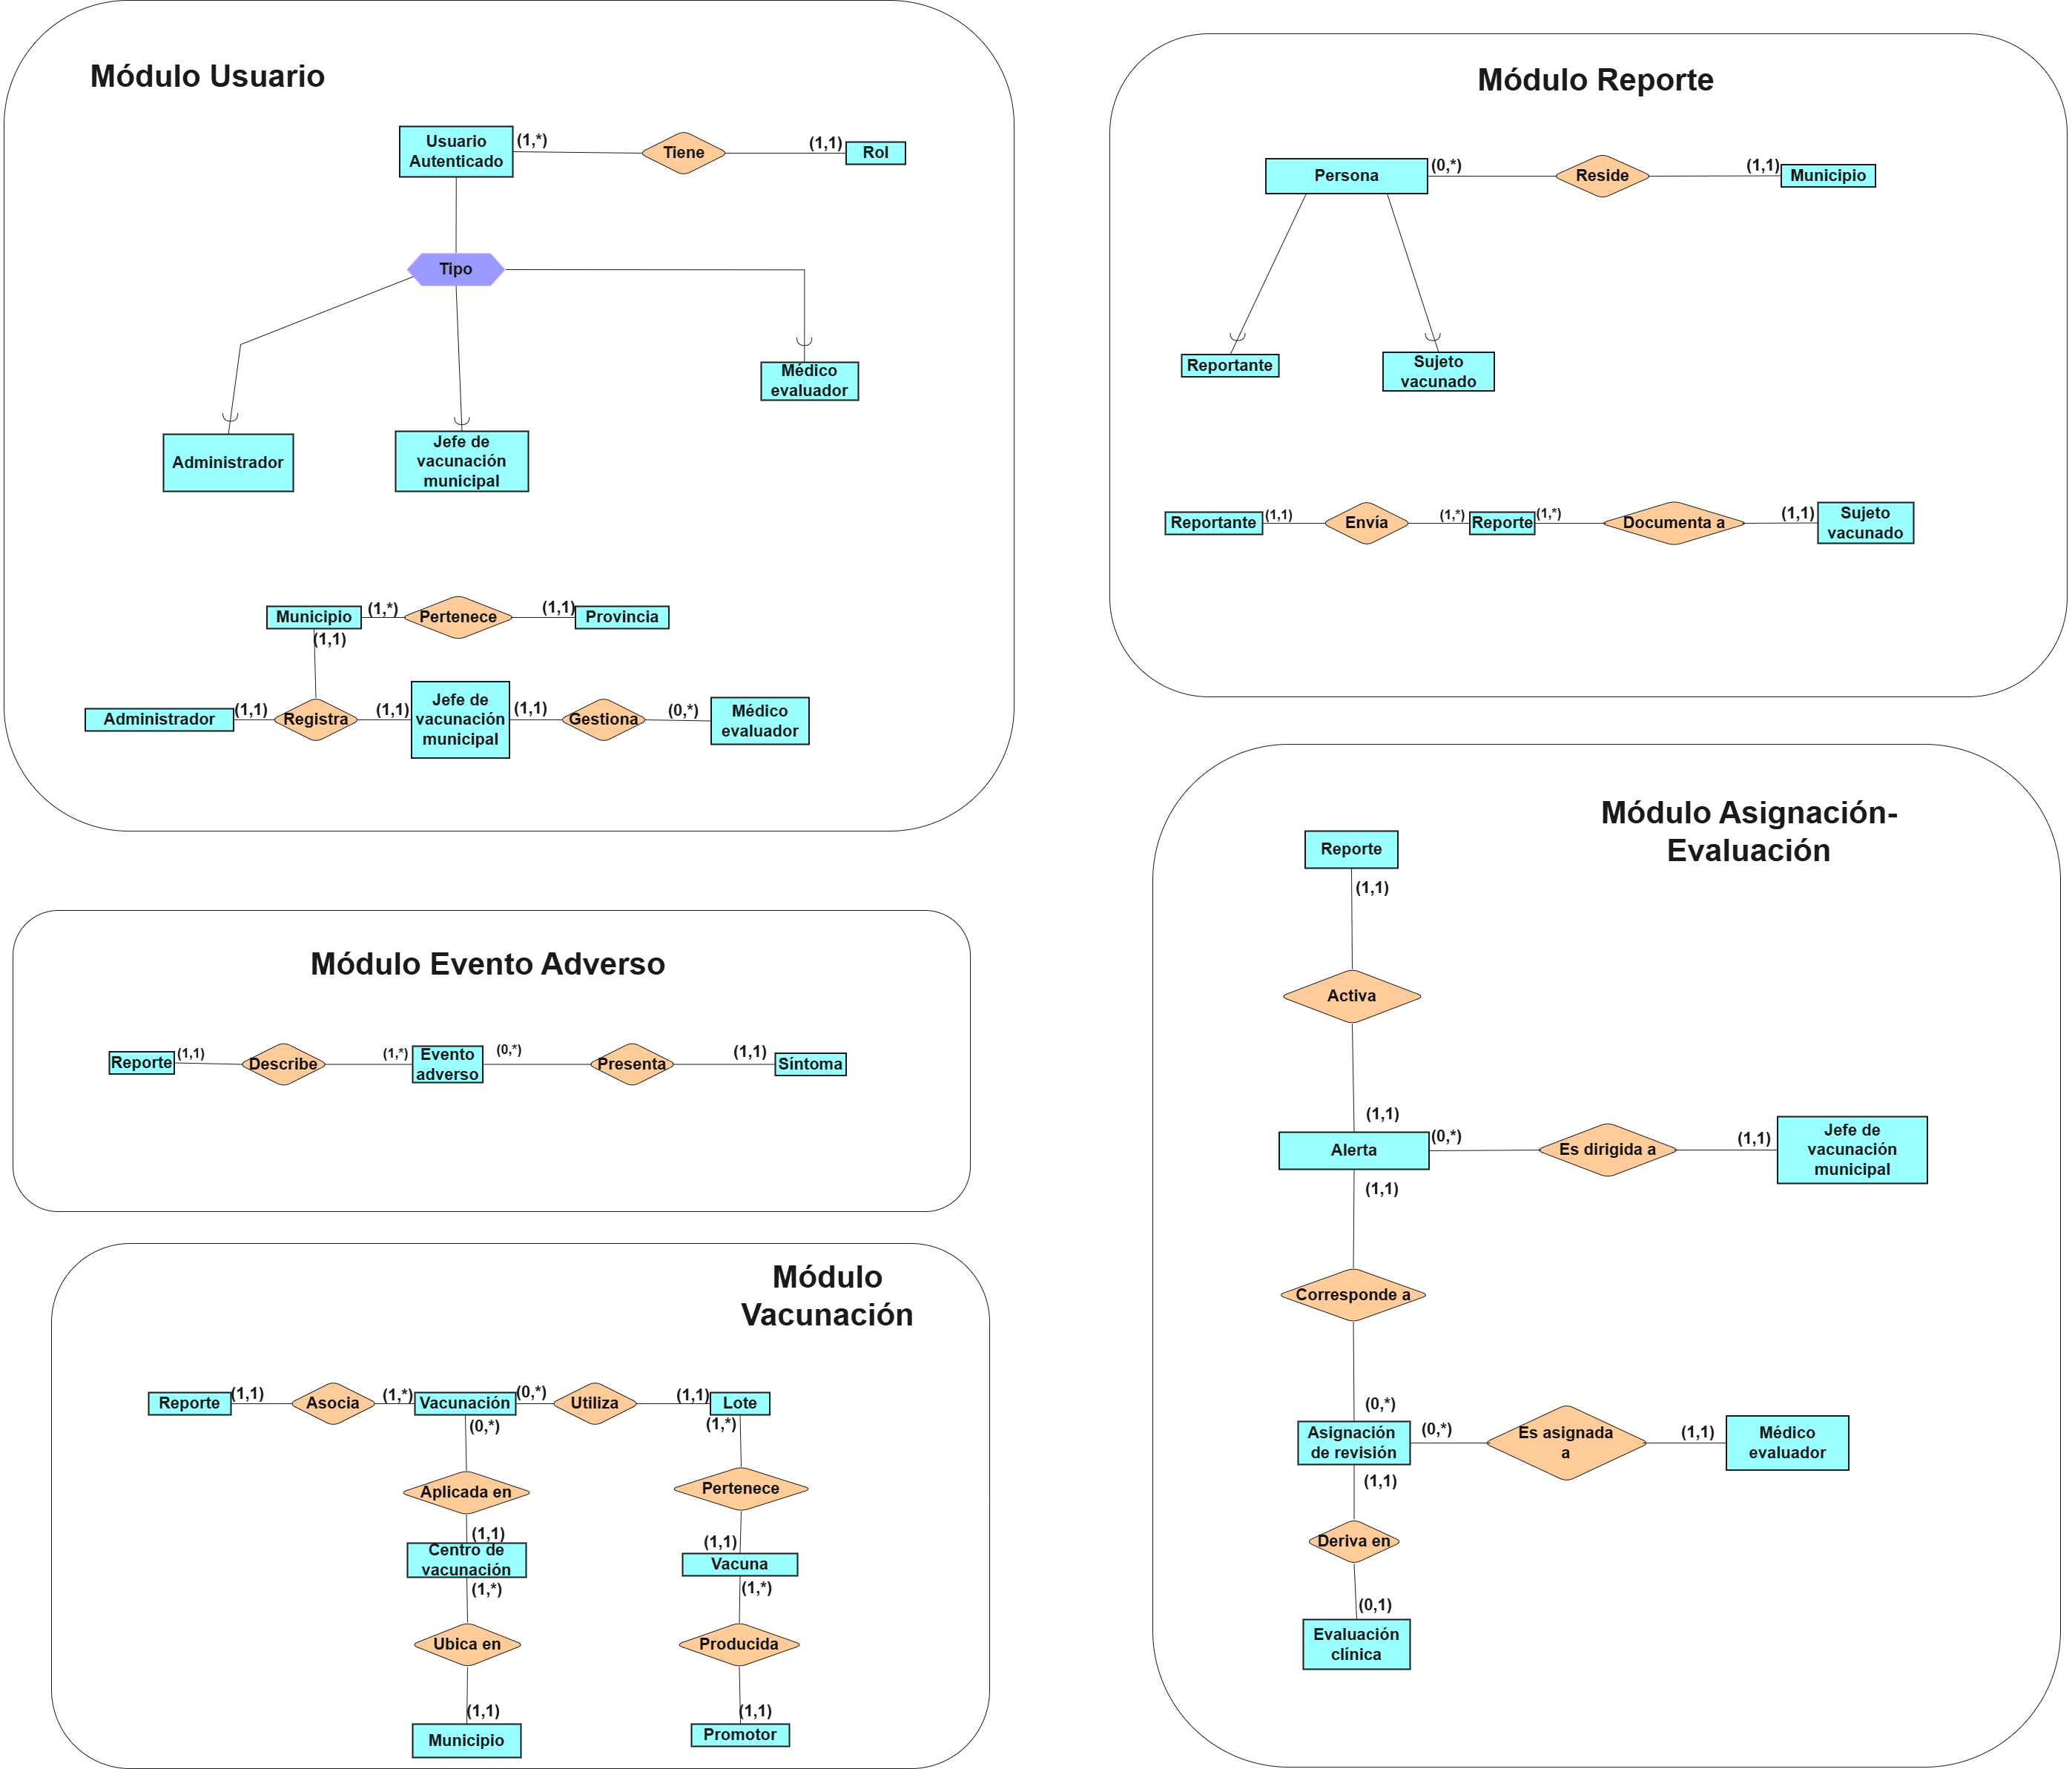
\includegraphics{Graphics/merx-modular.drawio.png}
    \end{adjustbox}
    \caption{Diagrama de modelo entidad-relación extendido (MERX). Fuente: elaboración propia.}
    \label{fig:merx}
\end{figure}


El diseño se organiza en cinco módulos funcionales que segmentan las responsabilidades del sistema:

\begin{itemize}
    \item \textbf{Módulo 1: Gestión de Usuarios y Roles} — Base de seguridad y control de acceso. Incluye jerarquía de herencia con las tablas \texttt{Usuario}, \texttt{Administrador}, \texttt{Jefe de Vacunación Municipal} y \texttt{Médico Evaluador}.
    \item \textbf{Módulo 2: Gestión de Reportes} — Núcleo del sistema. Integra la información del sujeto vacunado y del reportante mediante la jerarquía de herencia basada en la entidad \texttt{Person}.
    \item \textbf{Módulo 3: Vacunación} — Documenta los productos biológicos administrados, lotes, fabricantes y centros de salud.
    \item \textbf{Módulo 4: Evento Adverso} — Registra las manifestaciones clínicas (síntomas) detectadas tras la inmunización.
    \item \textbf{Módulo 5: Asignación y Evaluación} — Coordina el flujo de trabajo posterior a la notificación, gestionando alertas, asignaciones y dictámenes clínicos.
\end{itemize}

Todas las entidades del esquema emplean un identificador único universal (UUID) compuesto por 32 dígitos hexadecimales y 4 guiones que suman 36 caracteres, permitiendo generar el identificador sin depender de una secuencia centralizada de base de datos. 
Las tablas \texttt{Provincia} y \texttt{Municipio} constituyen la única excepción: emplean enteros autoincrementales por tratarse de catálogos geográficos con pocos registros y alta estabilidad.

Para acelerar las consultas, el diseño incorpora índices sobre campos de alta concurrencia como estados de reporte, fechas de creación, número de identidad (blind index) e identificadores de búsqueda frecuente.

\begin{table}[H]
\centering
\caption{Entidades principales del dominio}
\label{tab:entities}
\begin{tabular}{|p{5.8cm}|p{9.2cm}|}
\hline
\textbf{Entidad} & \textbf{Descripción} \\ \hline
User & Usuarios del sistema con roles internos y credenciales para autenticación. \\ \hline
Person & Centraliza la identidad inmutable (nombre, género, número de identidad) de ciudadanos que pueden ser sujetos o reportantes. \\ \hline
Admin / SectionResponsible / MedicalEvaluator & Especializaciones de usuario con permisos y responsabilidades específicas. \\ \hline
Reporter & Información del reportante, incluyendo datos de contacto obligatorios. \\ \hline
AefiReport & Reporte principal del evento ESAVI, con número de notificación único. \\ \hline
VaccinatedSubject & Datos del sujeto vacunado (hereda de Person). \\ \hline
Vaccination & Información sobre la vacuna administrada, lote, fabricante y centro de vacunación. \\ \hline
Vaccine / Symptom / Lot / Manufacturer / VaccinationCenter & Catálogos de apoyo para la captura del reporte. \\ \hline
MedicalReviewAssignment & Registro de asignación de revisión médica de un reporte. \\ \hline
ReportDuplicate & Información sobre reportes duplicados o potencialmente relacionados. \\ \hline
Alert & Notificaciones automáticas generadas para jefes municipales sobre nuevos reportes. \\ \hline
Evaluation & Dictamen clínico final registrado por el médico evaluador, con escala de causalidad WHO-UMC. \\ \hline
\end{tabular}
\end{table}

\subsection{Estrategia de respaldo}

Actualmente, en el entorno de desarrollo, los respaldos se gestionan de forma manual mediante la herramienta \texttt{mysqldump}, generando copias completas de la base de datos bajo demanda. 
Esta estrategia es suficiente para la fase actual de desarrollo y pruebas, donde el volumen de datos es reducido y los riesgos de pérdida son bajos. 
Para la puesta en producción, se establecerá un proceso automatizado que incluya respaldos programados diarios, retención por un período mínimo de 7 días y almacenamiento en ubicación externa a la base de datos productiva.













\section{API e Integraciones}

\subsection{Diseño de API}

El backend expone una API REST documentada con Swagger. Los controladores están agrupados por dominio, como Authentication, Report, Catalog, VaccinationCenter, MedicalReview y Dashboard. El frontend consume estos endpoints a través de un cliente Axios centralizado, que además maneja refresh de tokens y tratamiento de errores.

\subsection{Documentación de endpoints}

Ejemplo de endpoints del sistema:

\begin{lstlisting}
POST /api/Authentication/login
Descripción: Autentica un usuario y devuelve tokens de acceso y refresh.

POST /api/Report/createPublic
Descripción: Crea un reporte ESAVI de forma pública desde el frontend.

GET /api/Report/get-report
Descripción: Recupera el detalle de un reporte a partir de un identificador.

GET /api/GetCatalog/vaccines/actives
Descripción: Devuelve las vacunas activas para el formulario de reporte.

GET /api/VaccinationCenter/getByMunicipality
Descripción: Recupera los centros de vacunación asociados a una provincia y municipio.
\end{lstlisting}

\subsection{Integraciones externas}

\begin{table}[H]
\centering
\caption{Integraciones externas}
\label{tab:integraciones}
\begin{tabular}{|l|p{3.2cm}|p{8cm}|}
\hline
\textbf{Servicio} & \textbf{Tipo} & \textbf{Datos intercambiados} \\ \hline
FriendlyCaptcha & Captcha en formularios & Validación de humanidad en formularios públicos \\ \hline
EmailJS & Envío de correos electrónicos & Notificaciones a usuarios y reportantes sobre estados de reportes \\ \hline
MySQL & Base de datos relacional & Persistencia de reportes, usuarios y catálogos \\ \hline
RabbitMQ & Mensajería & Integración asíncrona y procesamiento de eventos \\ \hline
\end{tabular}
\end{table}














\section{Pruebas Funcionales}

\subsection{Estrategia de pruebas funcionales}

La validación de las funcionalidades críticas del sistema ESAVI se realizó mediante pruebas de caja negra, simulando operaciones de usuarios normales desde el navegador con datos sintéticos para verificar la persistencia y la respuesta del sistema ante entradas representativas.

La tabla \ref{tab:pruebas_funcionales} resume el estado de cumplimiento de las funciones principales: todos los casos de prueba seleccionados resultaron exitosos, confirmando la operatividad de la plataforma.

\begin{table}[H]
\centering
\caption{Resumen de casos de prueba funcionales}
\label{tab:pruebas_funcionales}
\begin{tabular}{|c|p{3.5cm}|p{2.5cm}|c|}
\hline
\textbf{ID} & \textbf{Caso de prueba} & \textbf{Tipo} & \textbf{Resultado} \\ \hline
CP01 & Inicio de sesión con credenciales válidas & Positivo & \checkmark \\ \hline
CP02 & Registro de reporte ESAVI con datos completos & Positivo & \checkmark \\ \hline
CP03 & Consulta por número de notificación existente & Positivo & \checkmark \\ \hline
CP04 & Gestión de usuarios (médico o jefe de sección) & Positivo & \checkmark \\ \hline
CP05 & Asignación de reporte a médico & Positivo & \checkmark \\ \hline
CP06 & Resolución de reportes duplicados & Positivo & \checkmark \\ \hline
CP07 & Visualización del dashboard administrativo & Positivo & \checkmark \\ \hline
CP08 & Filtrado de reportes & Positivo & \checkmark \\ \hline
CP09 & Revisión médica del reporte & Positivo & \checkmark \\ \hline
CP10 & Inicio de sesión con credenciales inválidas & Negativo & \checkmark \\ \hline
CP11 & Registro de reporte con datos obligatorios ausentes & Negativo & \checkmark \\ \hline
CP12 & Consulta de número de notificación inexistente & Negativo & \checkmark \\ \hline
\end{tabular}
\end{table}

\subsection{Evidencias de ejecución}

Esta sección presenta capturas de pantalla que evidencian la ejecución correcta de los principales flujos del sistema, validando la interacción entre el usuario y la interfaz.

\subsubsection{Flujo completo del manejo de reportes ESAVI}

Este flujo describe el ciclo completo de gestión de un reporte ESAVI, desde su creación por el usuario hasta su evaluación final por el médico evaluador y la consulta del estado actualizado del caso, tal como aparece en la figura~\ref{fig:esavi-flow}.

\begin{figure}[H]
    \centering
    \begin{subfigure}{0.45\textwidth}
        \centering
        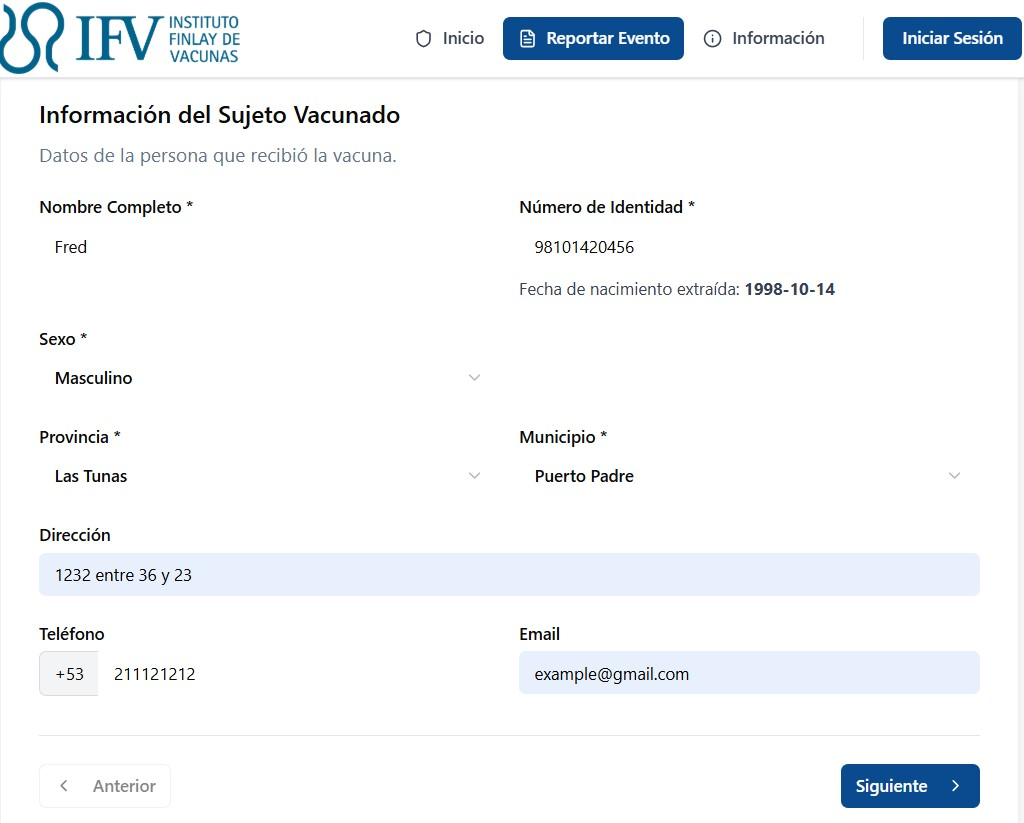
\includegraphics[width=\linewidth]{Cap5/creacion_reporte.jpg}
        \caption{Creación de reporte ESAVI}
    \end{subfigure}
    \hfill
    \begin{subfigure}{0.45\textwidth}
        \centering
        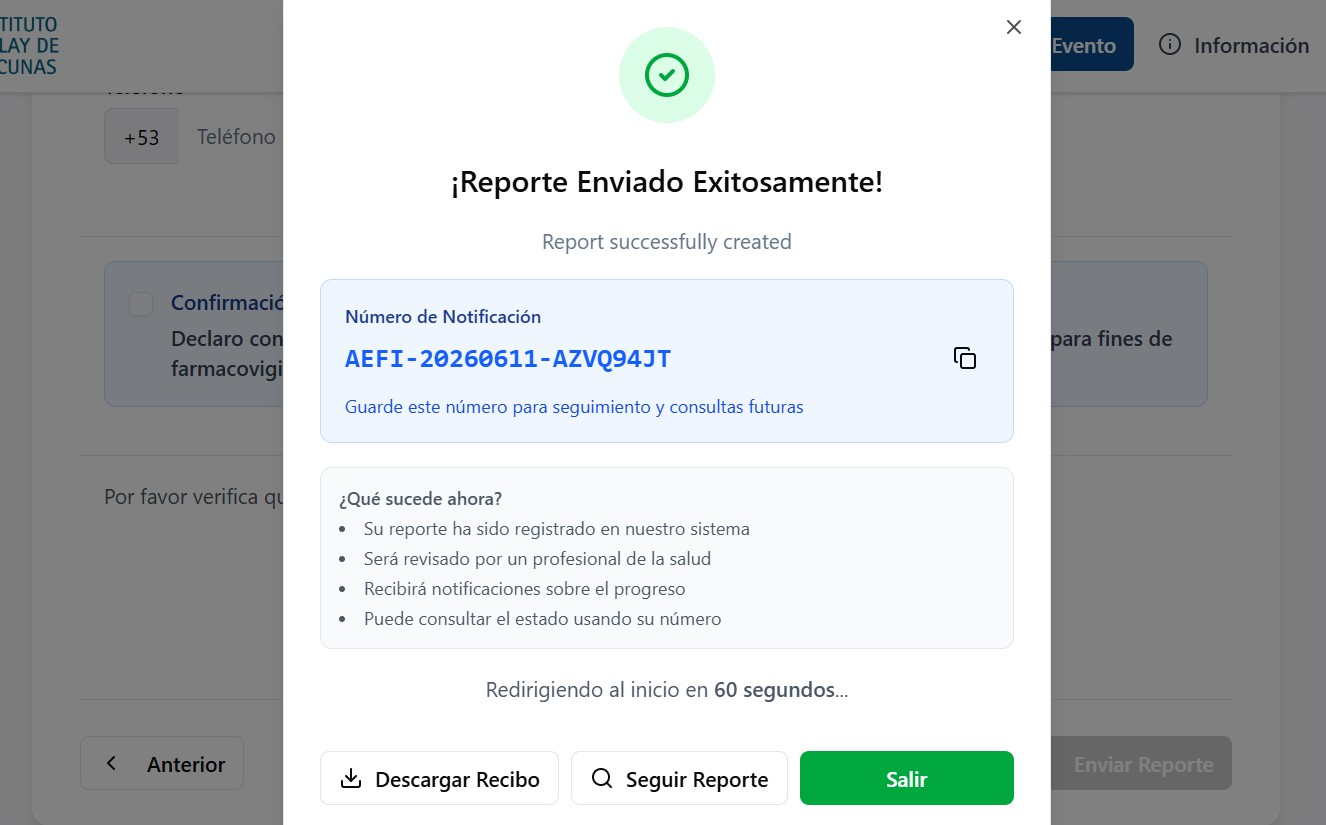
\includegraphics[width=\linewidth]{Cap5/creacion_reporte_exitoso.jpg}
        \caption{Confirmación de registro del reporte}
    \end{subfigure}

    \vspace{0.6cm}

    \begin{subfigure}{0.8\textwidth}
        \centering
        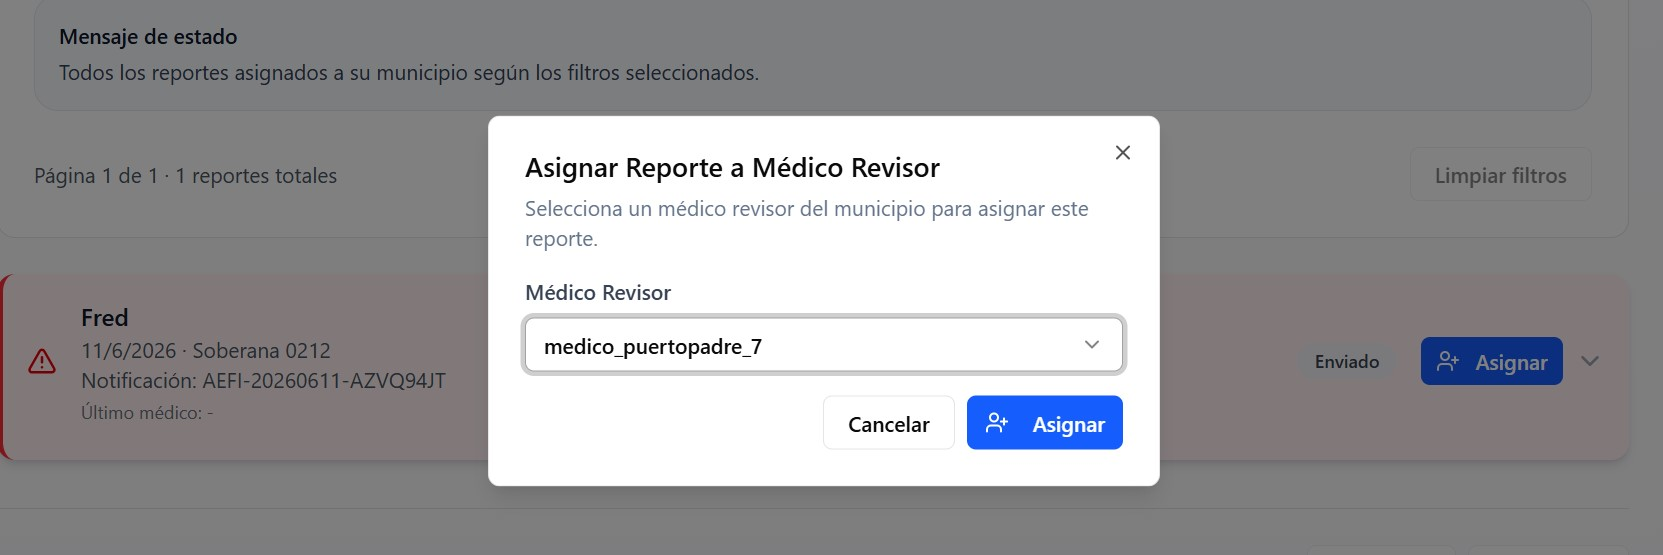
\includegraphics[width=\linewidth]{Cap5/captura_asignacion_jefe.jpg}
        \caption{Asignación del reporte por el jefe de vacunación municipal a un médico evaluador}
    \end{subfigure}

    \vspace{0.6cm}

    \begin{subfigure}{0.45\textwidth}
        \centering
        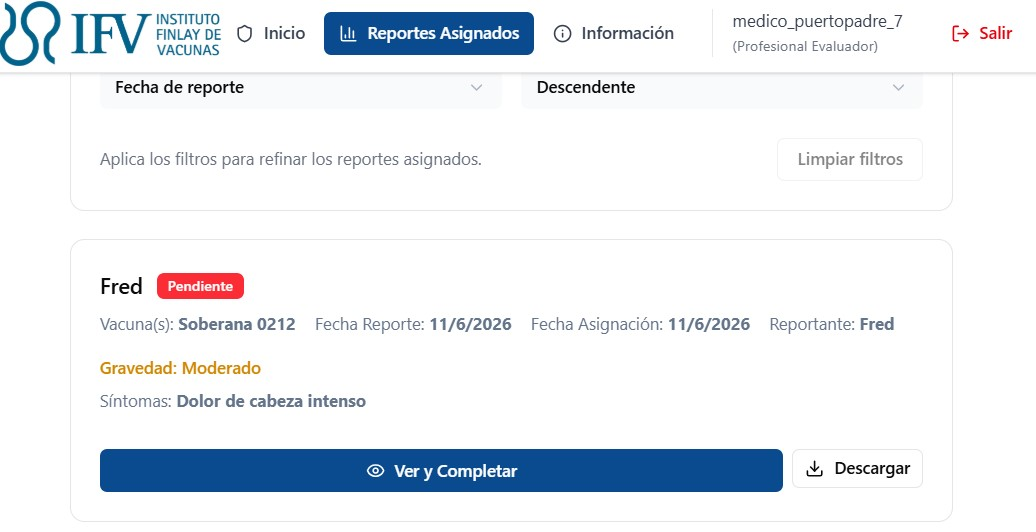
\includegraphics[width=\linewidth]{Cap5/asignación_vista.jpg}
        \caption{Visualización del reporte por el médico evaluador asignado}
    \end{subfigure}
    \hfill
    \begin{subfigure}{0.45\textwidth}
        \centering
        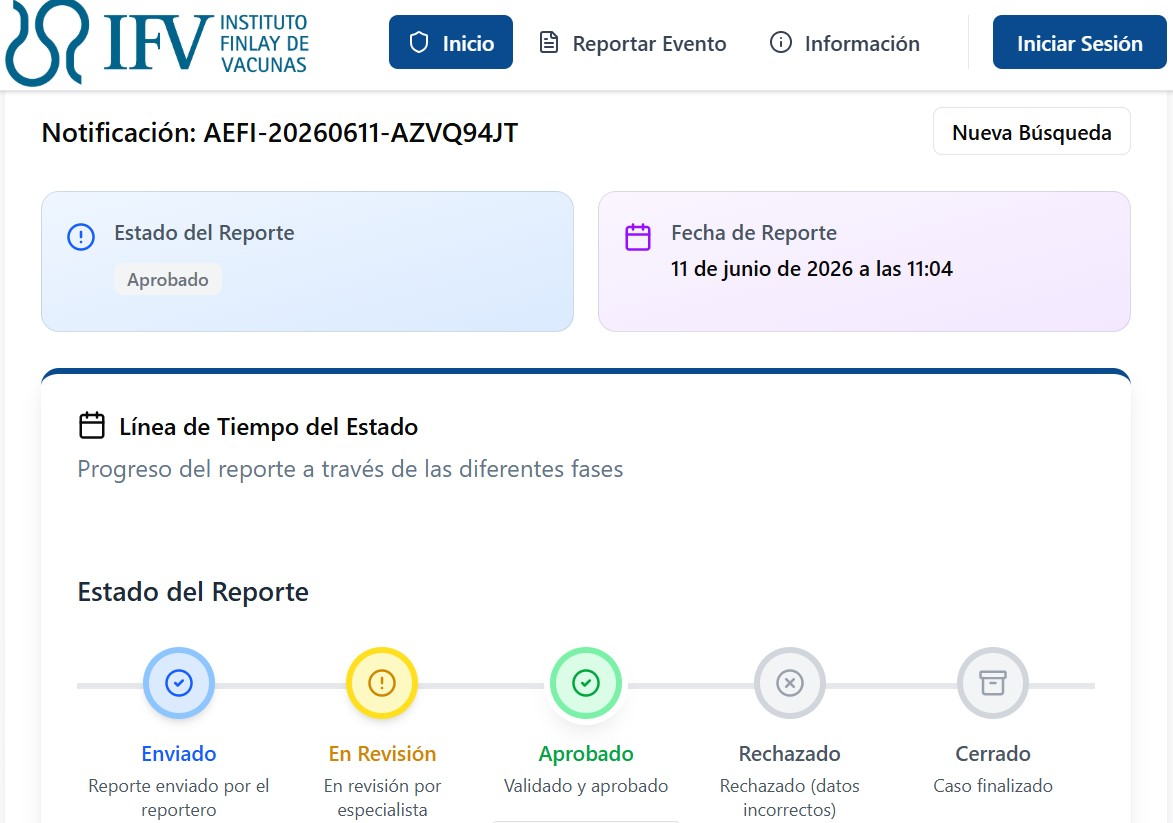
\includegraphics[width=\linewidth]{Cap5/busqueda_reporte2.jpg}
        \caption{Actualización del estado del reporte tras la evaluación médica}
    \end{subfigure}

    \caption{Flujo del sistema ESAVI para la creación, asignación y evaluación de reportes de eventos adversos posteriores a la vacunación}
    \label{fig:esavi-flow}
\end{figure}

\subsubsection{Gestión de acceso y registro de médico evaluador}

Este flujo, ilustrado en la figura \ref{fig:esavi-flow2}, abarca el registro de un médico evaluador por parte del jefe municipal, el envío de una invitación por correo electrónico, el establecimiento de contraseña y el posterior inicio de sesión en el sistema, garantizando un acceso controlado al módulo de revisión de reportes.

\begin{figure}[H]
    \centering
    \begin{subfigure}{0.45\textwidth}
        \centering
        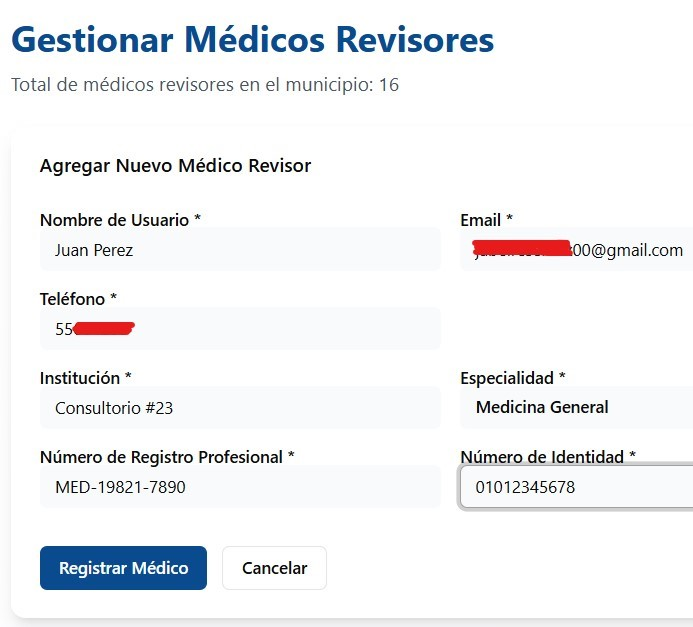
\includegraphics[scale=0.66]{Cap5/registro_médico2.jpg}
        \caption{Registro de médico evaluador por el jefe municipal}
    \end{subfigure}
    \hfill
    \begin{subfigure}{0.45\textwidth}
        \centering
        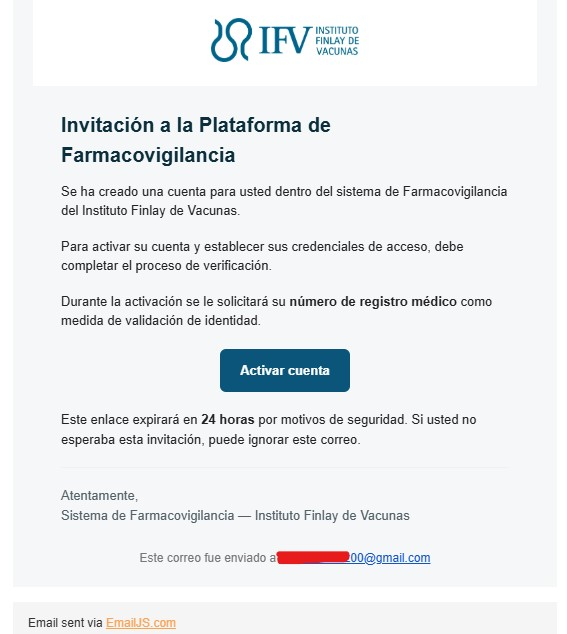
\includegraphics[width=\linewidth]{Cap5/correo_envio.jpg}
        \caption{Correo de invitación con enlace para establecer contraseña}
    \end{subfigure}

    \vspace{0.6cm}

    \begin{subfigure}{0.45\textwidth}
        \centering
        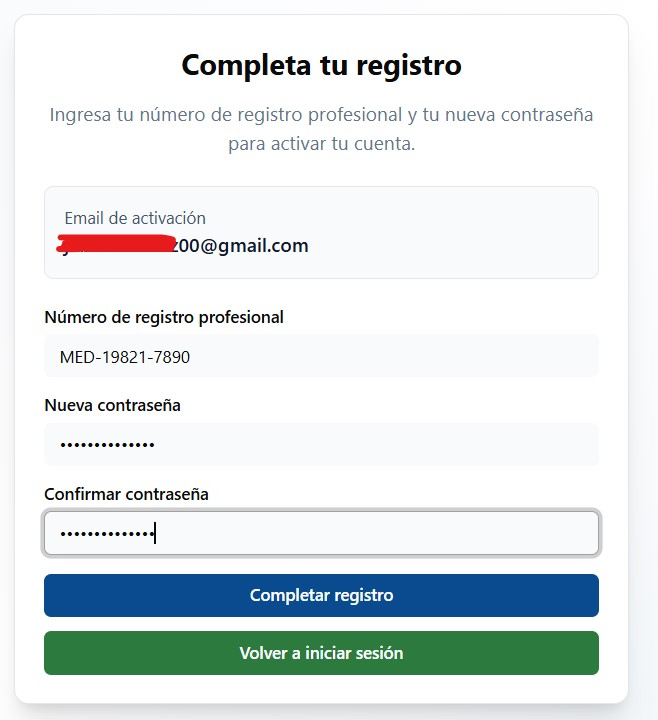
\includegraphics[width=\linewidth]{Cap5/correo_login.jpg}
        \caption{Página de establecimiento de contraseña}
    \end{subfigure}
    \hfill
    \begin{subfigure}{0.45\textwidth}
        \centering
        
\includegraphics[scale=0.5]{Cap5/login_exitoso.jpg}
        \caption{Pantalla de inicio tras autenticación exitosa}
    \end{subfigure}

    \caption{Flujo de registro y activación de un médico evaluador en el sistema ESAVI}
    \label{fig:esavi-flow2}
\end{figure}

\subsection{Análisis de resultados}

Los 12 casos de prueba funcionales fueron ejecutados con éxito, sin desviaciones entre los resultados esperados y los obtenidos. Los flujos principales —creación, asignación, revisión y consulta de reportes— operaron de extremo a extremo conforme a los requerimientos. El registro y activación de médicos evaluadores confirmó el control de acceso al sistema, y los casos negativos validaron que el sistema rechaza correctamente entradas inválidas. En conjunto, las pruebas funcionales demuestran que las funcionalidades críticas del sistema operan correctamente.
















\section{Rendimiento y Escalabilidad}

\subsection{Métricas de rendimiento}

Las pruebas de rendimiento se ejecutaron con k6, evaluando las operaciones críticas del sistema en diferentes escenarios de carga. La tabla \ref{tab:slo} define los objetivos de rendimiento establecidos para el sistema en condiciones normales de operación.

\begin{table}[H]
\centering
\caption{Objetivos de rendimiento (SLOs)}
\label{tab:slo}
\begin{tabular}{|l|l|l|l|}
\hline
\textbf{Métrica} & \textbf{Objetivo} & \textbf{Alerta} & \textbf{Crítico} \\ \hline
Latencia p95 & < 1000 ms & 2000 ms & 3000 ms \\ \hline
Throughput & 20 req/s & 15 req/s & 10 req/s \\ \hline
Tasa de éxito & 99.9\% & 99\% & 95\% \\ \hline
Solicitudes < umbral & 100\% & 95\% & 90\% \\ \hline
\end{tabular}
\end{table}

\subsection{Estrategia de escalabilidad}

El sistema fue diseñado con una arquitectura de monolito modular que permite las siguientes estrategias de escalabilidad:

\begin{itemize}
    \item \textbf{Vertical:} incremento de recursos (CPU, RAM) en el servidor que aloja el backend y la base de datos.
    \item \textbf{Horizontal:} replicación del backend mediante balanceo de carga, añadiendo instancias adicionales del servicio.
    \item \textbf{Caché:} implementación de caché distribuida (Redis) para reducir la carga en la base de datos.
    \item \textbf{Optimización de consultas:} uso de índices en columnas de alta concurrencia como \texttt{notification\_number}.
\end{itemize}

\subsection{Pruebas de carga realizadas}

Las pruebas de carga emplearon k6 como herramienta de evaluación. Los escenarios ejecutados fueron:

\begin{itemize}
    \item \textbf{Prueba de estrés incremental:} aumento progresivo de usuarios virtuales (VUs) para identificar el punto de saturación del sistema.
    \item \textbf{Prueba de volumen:} evaluación del impacto del crecimiento de la base de datos (1,000 a 100,000 reportes) en el rendimiento de búsqueda.
    \item \textbf{Escenario combinado:} simulación de carga realista con múltiples perfiles de usuario (ciudadanos, jefes municipales y médicos) operando simultáneamente.
\end{itemize}

\subsubsection{Resultados: Creación de reportes}

La prueba de estrés sobre la creación de reportes incrementó la carga desde 5 hasta 200 usuarios concurrentes. La tabla \ref{tab:creacion-resultados} resume los resultados obtenidos.

\begin{table}[H]
\centering
\caption{Resultados de creación de reportes}
\label{tab:creacion-resultados}
\begin{tabular}{|c|c|c|c|}
\hline
\textbf{VUs} & \textbf{Latencia p95 (ms)} & \textbf{Latencia promedio (ms)} & \textbf{\% < 3000 ms} \\ \hline
5 & 172.8 & 102.7 & 100\% \\ \hline
10 & 315.8 & 182.5 & 100\% \\ \hline
30 & 623.7 & 298.5 & 100\% \\ \hline
50 & 1158.1 & 530.8 & 100\% \\ \hline
70 & 2147.0 & 952.0 & 100\% \\ \hline
80 & 2851.3 & 1810.4 & 95.8\% \\ \hline
100 & 4033.2 & 2228.2 & 74.8\% \\ \hline
150 & 6706.2 & 4703.1 & 19.1\% \\ \hline
200 & 8005.9 & 5393.7 & 10.7\% \\ \hline
\end{tabular}
\end{table}

\begin{itemize}
    \item \textbf{Zona óptima:} Hasta 70 VUs, la latencia p95 se mantiene por debajo de 3000 ms.
    \item \textbf{Zona de degradación:} A partir de 80 VUs, la latencia comienza a superar los 2000 ms.
    \item \textbf{Throughput:} Se estabilizó entre 20 y 26 req/s en todos los niveles de carga.
    \item \textbf{Tasa de éxito:} 100\% de solicitudes exitosas (status 201) en todos los niveles.
\end{itemize}

\subsubsection{Resultados: Búsqueda de reportes}

La prueba de búsqueda por número de notificación evaluó el impacto del volumen de datos en la latencia, variando el tamaño de la base de datos desde 1,000 hasta 100,000 reportes.

\begin{table}[H]
\centering
\caption{Resultados de búsqueda por notificación (p95 en ms)}
\label{tab:busqueda-resultados}
\begin{tabular}{|c|c|c|c|c|c|}
\hline
\textbf{VUs} & \textbf{$10^3$} & \textbf{$4 \times 10^3$} & \textbf{$10^4$} & \textbf{$5 \times 10^4$} & \textbf{$10^5$} \\ \hline
5 & 48.4 & 79.6 & 55.4 & 85.3 & 110.5 \\ \hline
10 & 94.6 & 108.1 & 111.0 & 145.2 & 185.8 \\ \hline
30 & 320.2 & 358.1 & 354.5 & 430.7 & 520.3 \\ \hline
50 & 553.8 & 624.6 & 723.9 & 780.4 & 950.6 \\ \hline
70 & 787.9 & 830.2 & 862.2 & 1050.8 & 1350.2 \\ \hline
100 & 1073.4 & 1200.0 & 1540.4 & 1750.3 & 2200.7 \\ \hline
150 & 1637.2 & 1777.9 & 2027.3 & 2600.5 & 3100.4 \\ \hline
200 & 2425.2 & 2377.3 & 2951.4 & 3250.0 & 3850.0 \\ \hline
\end{tabular}
\end{table}

\begin{itemize}
    \item Hasta 70 VUs, todas las curvas permanecen agrupadas por debajo de 1500 ms.
    \item Con $10^3$, $4 \times 10^3$ y $10^4$ reportes, el umbral de 3000 ms no se supera incluso con 200 VUs.
    \item Con $5 \times 10^4$ y $10^5$ reportes, se supera el umbral a partir de 200 VUs.
    \item Tasa de éxito: 100\% de solicitudes exitosas (status 202) en todos los niveles.
\end{itemize}

\subsubsection{Resultados: Escenario combinado}

El escenario combinado simuló una carga realista con 100 VUs distribuidos en tres perfiles: 75 ciudadanos, 10 jefes municipales y 15 médicos evaluadores.

\begin{table}[H]
\centering
\caption{Métricas globales del escenario combinado}
\label{tab:metricas-globales}
\begin{tabular}{|l|c|}
\hline
\textbf{Métrica} & \textbf{Valor} \\ \hline
Solicitudes totales & 2,382 \\ \hline
Throughput global & 36.8 req/s \\ \hline
Latencia promedio global & 646.2 ms \\ \hline
Mediana global & 471.8 ms \\ \hline
p(95) global & 1623.4 ms \\ \hline
Tasa de éxito & 99.5\% \\ \hline
\end{tabular}
\end{table}

\begin{table}[H]
\centering
\caption{Métricas por operación en escenario combinado}
\label{tab:metricas-operaciones}
\footnotesize
\begin{tabular}{|l|c|c|c|c|c|}
\hline
\textbf{Operación} & \textbf{Solicitudes} & \textbf{Mediana (ms)} & \textbf{p95 (ms)} & \textbf{Outliers} \\ \hline
Crear reporte & 1078 & 858.28 & 2468.39 & 80 \\ \hline
Buscar reporte & 581 & 235.99 & 551.48 & 25 \\ \hline
Pendientes & 84 & 364.01 & 1143.59 & 8 \\ \hline
Médicos & 84 & 222.53 & 637.15 & 4 \\ \hline
Asignar & 84 & 433.23 & 1805.32 & 12 \\ \hline
Asignaciones & 365 & 278.22 & 783.83 & 18 \\ \hline
Evaluar & 68 & 382.17 & 911.90 & 4 \\ \hline
Dashboard & 38 & 368.06 & 1209.34 & 4 \\ \hline
\end{tabular}
\end{table}

\subsection{Resumen de resultados}

\begin{table}[H]
\centering
\caption{Resumen de resultados de rendimiento}
\label{tab:resumen-rendimiento}
\begin{tabular}{|l|l|l|}
\hline
\textbf{Operación} & \textbf{Capacidad máxima} & \textbf{p95 en carga normal} \\ \hline
Creación de reporte & 70 VUs sin degradación & 1158 ms (50 VUs) \\ \hline
Búsqueda por notificación & 200 VUs con $10^4$ reportes & 2951 ms (200 VUs, $10^4$) \\ \hline
Escenario combinado & 100 VUs & 1623 ms (global) \\ \hline
\end{tabular}
\end{table}

El sistema demuestra un rendimiento robusto bajo carga concurrente. Las pruebas de estrés establecen que el sistema soporta hasta 70 usuarios concurrentes en operaciones de escritura sin degradación significativa, y más de 100 usuarios en escenarios mixtos. El throughput se estabiliza en aproximadamente 25 req/s para operaciones de escritura y 37 req/s en escenarios combinados. La búsqueda por número de notificación es la operación mejor optimizada, gracias al índice B-Tree implementado en la base de datos.
















	\section{Seguridad}

\subsection{Autenticación basada en JWT y Refresh Token}

El sistema emplea JSON Web Tokens (JWT) como mecanismo de autenticación sin estado, combinado con tokens de actualización (refresh tokens) almacenados en cookies HttpOnly. Esta combinación responde a dos objetivos contrapuestos: el token de acceso tiene una vida útil corta para limitar el daño en caso de robo, pero el usuario no necesita iniciar sesión repetidamente.

\subsubsection{JSON Web Token (JWT)}

Un JWT es un estándar abierto definido en el RFC 7519 que permite transmitir información verificable entre dos partes mediante un token firmado digitalmente \cite{rfc7519}. El token consta de tres secciones codificadas en Base64 y separadas por puntos: encabezado, carga útil y firma. La carga útil contiene los \textit{claims} —afirmaciones sobre el usuario, como su identificador, nombre y rol—, mientras que la firma garantiza que el token no fue alterado desde su emisión.

El sistema genera el JWT mediante HMAC-SHA256 como algoritmo de firma con una clave secreta simétrica almacenada en variables de entorno. Esta clave nunca aparece en el código fuente ni llega al cliente. El token incluye cuatro claims: identificador del usuario, nombre de usuario, identificador único del token y rol del usuario. La expiración queda configurada en 15 minutos.

El middleware de ASP.NET Core valida cada solicitud entrante verificando que el emisor y la audiencia coincidan con los valores configurados, que la firma sea correcta y que el token no haya expirado.

\subsubsection{Refresh Token en cookie HttpOnly}

Para compensar la corta vida del JWT sin sacrificar seguridad, el sistema implementa refresh tokens. Un refresh token es un valor aleatorio generado criptográficamente mediante \texttt{RandomNumberGenerator} de .NET, que produce 64 bytes de entropía y los codifica en Base64. Este valor reside en la base de datos junto con su fecha de vencimiento (8 horas) y el identificador del usuario.

El refresh token se transmite en una cookie con las siguientes propiedades de seguridad:

\begin{table}[H]
\centering
\caption{Configuración de seguridad de la cookie del refresh token}
\label{tab:cookie-config}
\begin{tabular}{|l|p{10cm}|}
\hline
\textbf{Propiedad} & \textbf{Propósito} \\ \hline
\texttt{HttpOnly = true} & Impide que JavaScript acceda al token, neutralizando ataques XSS \\ \hline
\texttt{Secure = true} & Restringe la transmisión a conexiones HTTPS \\ \hline
\texttt{SameSite = None} & Permite envío desde dominios distintos (frontend/backend separados) \\ \hline
\texttt{Expires = 8h} & Caducidad del refresh token \\ \hline
\end{tabular}
\end{table}

Además, cada vez que el cliente utiliza un refresh token para obtener un nuevo JWT, el sistema aplica rotación: revoca el token anterior y emite uno nuevo. Si un atacante logra robar un refresh token, la rotación limita su utilidad a una única renovación.

\subsection{Autorización basada en roles (RBAC)}

Una vez que el middleware de autenticación valida el JWT y establece la identidad del usuario, el sistema delega el control de acceso en el atributo \texttt{[Authorize]} para restringir rutas por rol. El atributo \texttt{[Authorize(Roles = "SectionResponsible")]} indica al middleware de autorización que solo los usuarios cuyo claim \texttt{Role} coincida con ese valor pueden ejecutar el método.

La tabla \ref{tab:rbac} define la matriz de permisos según el rol del usuario:

\begin{table}[H]
\centering
\caption{Matriz de permisos (RBAC)}
\label{tab:rbac}
\begin{tabular}{|l|c|c|c|c|}
\hline
\textbf{Recurso/Acción} & \textbf{Admin} & \textbf{SectionResponsible} & \textbf{MedicalEvaluator} & \textbf{Guest} \\ \hline
Usuarios - Gestionar & Sí & No & No & No \\ \hline
Reportes - Crear & Sí & Sí & No & Sí \\ \hline
Reportes - Ver todos & Sí & Sí & No & No \\ \hline
Reportes - Ver asignados & Sí & Sí & Sí & No \\ \hline
Reportes - Editar & Sí & Sí & Sí & No \\ \hline
Asignar médicos & Sí & Sí & No & No \\ \hline
Evaluar reportes & Sí & No & Sí & No \\ \hline
Configuración del sistema & Sí & No & No & No \\ \hline
Consultar estado de reporte & Sí & Sí & Sí & Sí \\ \hline
\end{tabular}
\end{table}

Para que la capa de aplicación pueda acceder a la identidad del usuario autenticado sin que el frontend la envíe manualmente, el sistema implementa el servicio \texttt{UserContextService}. Este servicio extrae el claim \texttt{NameIdentifier} del token JWT validado —disponible en el \texttt{HttpContext} de la solicitud— y lo expone mediante el método \texttt{GetUserId()}. Este enfoque elimina la necesidad de que cada ruta reciba explícitamente el identificador del usuario como parámetro.

\subsection{Protección de datos sensibles}

\subsubsection{Hashing de contraseñas}

La documentación oficial de Microsoft describe que el \texttt{PasswordHasher} de Identity implementa el algoritmo PBKDF2 (Password-Based Key Derivation Function 2), estándar del RFC 2898 que deriva una clave segura a partir de una contraseña \cite{rfc2898}. 
El algoritmo toma la contraseña del usuario, la combina con un \textit{salt} criptográficamente aleatorio de 128 bits y aplica repetidamente la función HMAC-SHA256 durante 600,000 iteraciones como valor configurado \cite{microsoft_password_hasher}.

El formato del hash generado produce una cadena con la siguiente estructura:

\begin{center}
\texttt{Base64(salt).Base64(subkey)}
\end{center}

\begin{table}[H]
\centering
\caption{Propiedades de seguridad del mecanismo de hashing}
\label{tab:hashing-propiedades}
\begin{tabular}{|l|p{10cm}|}
\hline
\textbf{Propiedad} & \textbf{Descripción} \\ \hline
Unicidad del hash & Dos usuarios con la misma contraseña producen hashes completamente diferentes por el \textit{salt} único \\ \hline
Irreversibilidad computacional & PBKDF2 es una función unidireccional; el elevado número de iteraciones ralentiza ataques por fuerza bruta \\ \hline
Invalidación de sesiones previas & La propiedad \texttt{SecurityStamp} invalida tokens anteriores al cambiar la contraseña \\ \hline
\end{tabular}
\end{table}

\subsubsection{Cifrado de datos sensibles y índice ciego}

Para armonizar la protección de datos sensibles con la necesidad de detectar reportes duplicados, la infraestructura implementa un índice ciego sobre el número de identidad del ciudadano.

La entidad persona almacena dos campos derivados del número de identidad:

\begin{itemize}
    \item \texttt{IdentityNumberEncrypted}: preserva el valor original mediante cifrado AES-256 para su recuperación clínica.
    \item \texttt{IdentityNumberBlindIndex}: contiene un hash HMAC-SHA256 generado con una clave criptográfica distinta de la usada para el cifrado. Esta columna porta un índice que permite al motor de base de datos localizar el registro en tiempo logarítmico.
\end{itemize}

\begin{table}[H]
\centering
\caption{Medidas de protección de datos}
\label{tab:proteccion-datos}
\begin{tabular}{|l|l|p{8cm}|}
\hline
\textbf{Medida} & \textbf{Estándar} & \textbf{Aplicación en el sistema} \\ \hline
En tránsito & TLS 1.2+ & HSTS, certificados válidos, conexiones HTTPS forzadas \\ \hline
En reposo & AES-256 & Cifrado a nivel de campo para números de identidad \\ \hline
Hashing de contraseñas & PBKDF2-SHA256 & 600,000 iteraciones, salt de 128 bits \\ \hline
Datos sensibles en logs & Enmascaramiento & Números de identidad y correos no se registran en texto plano \\ \hline
\end{tabular}
\end{table}

\subsection{Prevención de envíos duplicados (Idempotencia)}

Para evitar duplicados por dobles clics, reintentos automáticos por fallos de red o pérdidas de conectividad, la aplicación cliente implementa un mecanismo de idempotencia basado en una clave única asociada a cada operación de envío.

La clave surge de \texttt{crypto.randomUUID()}, función estandarizada que produce identificadores UUID v4 mediante un generador criptográficamente seguro. Una vez creada, la clave permanece almacenada en memoria del navegador hasta que el servidor responde satisfactoriamente.

El backend almacena la clave en una columna indexada con restricción de unicidad en la base de datos, lo que garantiza la creación de un único reporte incluso bajo escenarios de concurrencia extrema \cite{mysql_isolation}.

\subsection{Protección ante ataques automatizados}

\subsubsection{CAPTCHA}

Las rutas públicas del sistema —inicio de sesión, registro de reportes, consulta por número de notificación— están expuestas a ataques automatizados. 
Como primera barrera, el sistema exige que cada solicitud incluya un token de Friendly CAPTCHA, un servicio basado en prueba de trabajo (proof-of-work) que resuelve el desafío criptográfico en segundo plano sin interrumpir al usuario \cite{friendlycaptcha}.

Para integrar este servicio, es necesario crear una cuenta en el sitio oficial de Friendly CAPTCHA y registrar una nueva aplicación. El proceso genera dos claves:

\begin{itemize}
    \item \textbf{Sitekey}: identificador público que se incrusta en el frontend para inicializar el widget.
    \item \textbf{Secret key}: clave privada que se almacena exclusivamente en el backend para verificar los tokens recibidos.
\end{itemize}

Esta separación garantiza que el proceso de verificación solo pueda realizarse desde el backend, impidiendo que un atacante pueda falsificar tokens válidos \cite{friendlycaptcha}.

\subsubsection{Limitación de velocidad (Rate Limiting)}

La limitación de velocidad restringe el número de solicitudes que un cliente puede realizar a la API en un período de tiempo determinado. 
Su propósito es proteger el sistema contra ataques de fuerza bruta, enumeración de recursos y denegación de servicio \cite{microsoft_rate_limiting}.

\begin{table}[H]
\centering
\caption{Políticas de rate limiting configuradas}
\label{tab:rate-limiting}
\begin{tabular}{|l|l|l|l|}
\hline
\textbf{Política} & \textbf{Límite} & \textbf{Ventana} & \textbf{Aplicación} \\ \hline
Auth & 3 solicitudes & 1 minuto & Inicio de sesión \\ \hline
Command & 5 solicitudes & 1 minuto & Creación de reportes \\ \hline
ReportDaily & 30 solicitudes & 24 horas & Creación de reportes por IP \\ \hline
CommandDaily & 20 solicitudes & 24 horas & Operaciones administrativas \\ \hline
Query & 60 solicitudes & 1 minuto & Consultas y lecturas \\ \hline
\end{tabular}
\end{table}

\subsection{Gestión de secretos}

Las siguientes buenas prácticas se aplican para la gestión de secretos en el sistema:

\begin{itemize}
    \item \textbf{Nunca hardcodear secretos}: Las claves JWT, contraseñas de base de datos y credenciales de servicios externos se almacenan en variables de entorno.
    \item \textbf{Separación por entorno}: Existen conjuntos de variables diferentes para desarrollo, pruebas y producción.
    \item \textbf{Rotación de claves}: Las claves JWT pueden rotarse sin afectar a los usuarios activos.
    \item \textbf{Acceso restringido}: Solo personal autorizado tiene acceso a las variables de entorno de producción.
\end{itemize}

En producción, se recomienda adoptar soluciones más avanzadas como HashiCorp Vault o AWS Secrets Manager para la gestión centralizada de secretos.













	\section{Monitoreo y Logs}

\subsection{Estrategia de logging}

La capa de backend de ESAVI Report implementa un sistema de logging basado en Serilog, con salida simultánea a consola y archivos de log diarios. La configuración se realiza en el archivo \texttt{Program.cs} mediante \texttt{builder.Host.UseSerilog();}, junto con \texttt{WriteTo.Console()} y \texttt{WriteTo.File("logs/app-.log", rollingInterval: RollingInterval.Day)}. Esto permite mantener trazabilidad de eventos críticos, errores de validación, ejecuciones de servicios y fallas operativas durante la vida del sistema.

Los niveles configurados son:

\begin{itemize}
    \item \textbf{INFO}: Operaciones normales y flujos exitosos.
    \item \textbf{WARN}: Eventos inusuales que no impiden la operación.
    \item \textbf{ERROR}: Fallos recuperables que afectan una operación específica.
    \item \textbf{CRITICAL}: Fallos graves que requieren atención inmediata.
\end{itemize}

Cada entrada registra datos estructurados como timestamp, nivel, servicio, identificador de correlación, mensaje y metadatos de contexto, lo que facilita la búsqueda y el diagnóstico en entornos con múltiples peticiones concurrentes.

\subsection{Manejo centralizado de errores}

El sistema implementa un middleware de manejo de errores que captura excepciones no controladas y responde con un formato JSON uniforme, reduciendo la ambigüedad en auditoría y soporte. Este middleware registra automáticamente cada excepción en Serilog con el nivel apropiado y el contexto completo de la petición.

\subsection{Estado actual del monitoreo}

Actualmente, el sistema cuenta con las siguientes capacidades de observabilidad:

\begin{itemize}
    \item \textbf{Logs estructurados}: Implementados con Serilog en el backend.
    \item \textbf{Almacenamiento de logs}: Archivos rotativos diarios en el sistema de archivos.
    \item \textbf{Manejo de errores}: Middleware centralizado para excepciones no controladas.
    \item \textbf{Health checks}: \textit{Pendiente de implementación para la versión productiva.}
    \item \textbf{Métricas y alertas}: \textit{Pendiente de implementación.}
\end{itemize}

\subsection{Recomendaciones para el entorno productivo}

Para la puesta en producción, se recomienda implementar las siguientes mejoras:

\begin{table}[H]
    \centering
    \caption{Alertas propuestas para el entorno productivo}
    \label{tab:alertas}
    \begin{tabular}{|l|l|l|p{5cm}|}
        \hline
        \textbf{Métrica} & \textbf{Umbral} & \textbf{Severidad} & \textbf{Acción} \\ \hline
        CPU & $\ge$ 80\% (5 min sostenido) & Warning & Revisar procesos y escalar recursos \\ \hline
        Errores 5xx & $>$ 1\% (2 min sostenido) & Critical & Revisión inmediata del backend y logs \\ \hline
        Latencia p95 & $>$ 500 ms (10 min sostenido) & Warning & Optimizar consultas o escalar horizontalmente \\ \hline
        Memoria RAM & $>$ 85\% (5 min sostenido) & Warning & Analizar fugas de memoria y reiniciar servicio \\ \hline
        Disponibilidad & $<$ 99\% (5 min sostenido) & Critical & Alertar al equipo de operaciones \\ \hline
    \end{tabular}
\end{table}

Para la observabilidad en producción, se sugiere adoptar progresivamente herramientas como:

\begin{itemize}
    \item \textbf{Logs centralizados}: ELK Stack o Grafana Loki para agregar y consultar logs.
    \item \textbf{Métricas}: Prometheus + Grafana para almacenar y visualizar métricas.
    \item \textbf{APM}: New Relic o Datadog (opcional, según disponibilidad).
\end{itemize}

El siguiente paso de madurez operativa es centralizar los logs en un sistema de agregación y configurar dashboards que permitan correlacionar incidentes entre frontend, API y base de datos.













\section{Despliegue e Integración Continua}

\subsection{Estado actual del despliegue}

El sistema se despliega mediante contenedores Docker orquestados con Docker Compose. La arquitectura se compone de cuatro servicios principales:

\begin{table}[H]
\centering
\caption{Servicios del sistema}
\label{tab:servicios-despliegue}
\begin{tabular}{|l|l|l|}
\hline
\textbf{Servicio} & \textbf{Tecnología} & \textbf{Puerto} \\ \hline
API Backend & ASP.NET Core 8 & 5137 \\ \hline
Base de datos & MySQL 8.0 & 3306 \\ \hline
Mensajería & RabbitMQ 3-management & 5672 (AMQP), 15672 (UI) \\ \hline
Frontend & React + Vite + Nginx & 8080 \\ \hline
\end{tabular}
\end{table}

El backend se conecta a MySQL y RabbitMQ mediante variables de entorno definidas en \texttt{docker-compose.yml}. El frontend se sirve como una aplicación estática con Nginx.

\subsection{Pipeline CI/CD}

Actualmente, el repositorio no cuenta con pipelines de CI/CD automatizados. El despliegue se realiza de forma local mediante Docker Compose. Para producción, se recomienda incorporar un pipeline con las siguientes etapas:

\begin{itemize}
    \item \textbf{Build}: Compilación de frontend y backend.
    \item \textbf{Pruebas}: Ejecución de pruebas unitarias y de integración.
    \item \textbf{Análisis de seguridad}: Escaneo de vulnerabilidades en dependencias.
    \item \textbf{Despliegue}: Publicación en entornos de staging y producción.
\end{itemize}

Herramientas recomendadas: GitHub Actions, GitLab CI o Jenkins.

\subsection{Integración con servicios externos}

\begin{table}[H]
\centering
\caption{Servicios externos integrados}
\label{tab:servicios-externos}
\begin{tabular}{|l|l|p{5cm}|}
\hline
\textbf{Servicio} & \textbf{Propósito} & \textbf{Estado} \\ \hline
EmailJS & Envío de notificaciones por correo & Prototipo (reemplazar en producción) \\ \hline
OpenWA / WhatsApp & Envío de mensajes por WhatsApp & Prototipo (reemplazar en producción) \\ \hline
FriendlyCaptcha & Validación de humanidad en formularios & Integrado \\ \hline
\end{tabular}
\end{table}

Los servicios de notificación (EmailJS y OpenWA) operan como servicios externos a la infraestructura Docker. En producción, deben reemplazarse por soluciones institucionales (SMTP propio y WhatsApp Business API).

\subsection{Gestión de infraestructura}

La infraestructura se gestiona con un enfoque basado en contenedores y configuración declarativa:

\begin{table}[H]
\centering
\caption{Gestión de infraestructura}
\label{tab:infraestructura}
\begin{tabular}{|l|l|}
\hline
\textbf{Componente} & \textbf{Tecnología} \\ \hline
Orquestación & Docker Compose \\ \hline
Contenerización & Docker \\ \hline
Variables de entorno & Archivos \texttt{.env} \\ \hline
Migraciones & Entity Framework Core + \texttt{dotnet-ef} \\ \hline
Logs & Serilog (archivos diarios) \\ \hline
\end{tabular}
\end{table}

Para un despliegue productivo, se recomienda evolucionar hacia orquestadores más robustos (Docker Swarm o Kubernetes), externalizar la configuración sensible, aplicar health checks y automatizar la construcción de imágenes.

\subsection{Recomendaciones para producción}

\begin{enumerate}
    \item Migrar a servidores del Instituto Finlay (reemplazar Railway y Vercel).
    \item Configurar SMTP institucional y WhatsApp Business API.
    \item Implementar pipeline CI/CD automatizado.
    \item Establecer health checks y monitoreo con Prometheus + Grafana.
    \item Configurar respaldos automáticos de la base de datos.
\end{enumerate}








% \section{Mantenimiento y Soporte}

% \subsection{Plan de mantenimiento}

% El sistema ESAVI Report está organizado en dos componentes principales: un backend en .NET y un frontend en React con TypeScript, ambos desplegados con contenedores Docker.

% El plan de mantenimiento se estructura en cuatro líneas de acción:

% \begin{table}[H]
% \centering
% \caption{Líneas de mantenimiento}
% \label{tab:mantenimiento}
% \begin{tabular}{|p{3.5cm}|p{9cm}|}
% \hline
% \textbf{Tipo} & \textbf{Actividades} \\ \hline
% Correctivo & Corrección de errores funcionales en formularios, validaciones, asignaciones y notificaciones \\ \hline
% Adaptativo & Ajustes por cambios regulatorios, nuevos requerimientos de correo/WhatsApp y criterios de validación \\ \hline
% Perfectivo & Mejoras de usabilidad, optimización de rendimiento y ampliación de dashboards \\ \hline
% Preventivo & Revisión de dependencias, auditoría de logs, validación de respaldos y pruebas de regresión \\ \hline
% \end{tabular}
% \end{table}

% La operación se apoya en Serilog para logs estructurados, middleware de manejo de errores y limitación de peticiones. La infraestructura se gestiona con Docker Compose y scripts de migración.

% \subsection{Gestión de incidentes}

% La gestión de incidentes sigue el proceso: detección, clasificación, respuesta, resolución y cierre.

% \begin{table}[H]
% \centering
% \caption{Clasificación de incidentes}
% \label{tab:incidentes}
% \begin{tabular}{|c|p{5cm}|p{5cm}|}
% \hline
% \textbf{Prioridad} & \textbf{Descripción} & \textbf{Acción} \\ \hline
% P1 & Indisponibilidad crítica del sistema & Respuesta inmediata, activación de soporte \\ \hline
% P2 & Fallo funcional relevante & Revisión de logs, reproducción en entorno de prueba \\ \hline
% P3 & Error funcional puntual & Documentación y corrección planificada \\ \hline
% P4 & Solicitudes menores o mejoras & Planificación en siguiente ciclo \\ \hline
% \end{tabular}
% \end{table}

% Los eventos relacionados con autenticación, reportes ESAVI y notificaciones deben registrarse con contexto de usuario y operación. El cierre debe documentarse con un resumen ejecutivo y, cuando corresponda, un post-mortem.

% \subsection{Documentación de soporte}

% \begin{table}[H]
% \centering
% \caption{Documentación de soporte disponible}
% \label{tab:documentacion}
% \begin{tabular}{|p{4cm}|p{9cm}|}
% \hline
% \textbf{Recurso} & \textbf{Descripción} \\ \hline
% README.md & Finalidad del sistema y propósito institucional \\ \hline
% Manuales de despliegue & Instrucciones para compilar y levantar servicios (backend y frontend) \\ \hline
% Logs de backend & Trazabilidad de eventos y errores (Serilog, archivos diarios) \\ \hline
% Swagger/OpenAPI & Documentación y prueba de endpoints de la API \\ \hline
% Estructura por capas & Código organizado en dominio, aplicación, infraestructura y presentación \\ \hline
% \end{tabular}
% \end{table}

% Para producción, se recomienda complementar con runbooks, procedimientos de recuperación ante desastres y checklist de despliegue.







\section{Gestión de Riesgos}

\subsection{Identificación de riesgos}

La siguiente tabla identifica los principales riesgos técnicos y operativos identificados durante el desarrollo del sistema, junto con su impacto y probabilidad estimada.

\begin{table}[H]
\centering
\caption{Identificación de riesgos}
\label{tab:riesgos}
\begin{tabular}{|c|p{6cm}|c|c|}
\hline
\textbf{ID} & \textbf{Riesgo} & \textbf{Impacto} & \textbf{Probabilidad} \\ \hline
R001 & Dependencia de librerías mantenidas por una sola persona & Alto & Media \\ \hline
R002 & Base de datos podría no escalar adecuadamente & Alto & Baja \\ \hline
R003 & Fuga de datos por configuración incorrecta & Crítico & Media \\ \hline
R004 & Dependencia de conocimiento tácito de un desarrollador clave & Alto & Alta \\ \hline
R005 & Cambio inesperado en API de servicios externos (EmailJS, FriendlyCaptcha) & Alto & Media \\ \hline
\end{tabular}
\end{table}

\subsection{Planes de mitigación}

Para cada riesgo identificado, se han definido las siguientes estrategias de mitigación:

\begin{table}[H]
\centering
\caption{Planes de mitigación de riesgos}
\label{tab:mitigacion}
\begin{tabular}{|c|p{7cm}|p{5cm}|}
\hline
\textbf{ID} & \textbf{Estrategia de mitigación} & \textbf{Estado} \\ \hline
R001 & Evaluar alternativas y mantener versiones estables documentadas & En curso \\ \hline
R002 & Implementar índices en columnas críticas y planificar read replicas & Planificado \\ \hline
R003 & Auditorías automáticas de configuración, variables de entorno y logs & Implementado \\ \hline
R004 & Documentación obligatoria del código y arquitectura & En curso \\ \hline
R005 & Implementar capa de abstracción para servicios externos & Implementado \\ \hline
\end{tabular}
\end{table}

\subsection{Análisis de riesgos mitigados}

Los riesgos R003 (fuga de datos) y R005 (cambios en APIs externas) cuentan con mitigaciones ya implementadas en el sistema: el cifrado de datos sensibles mediante AES-256, el índice ciego y la capa de abstracción para servicios de notificación. Los riesgos R001 y R04 requieren acciones continuas de documentación y monitoreo de dependencias. El riesgo R002, aunque de baja probabilidad actualmente, debe ser monitoreado a medida que el sistema crezca en producción.











	\section{Accesibilidad y Experiencia de Usuario}

\subsection{Cumplimiento de accesibilidad}

El sistema ha sido evaluado en cumplimiento de los estándares WCAG 2.1 (niveles A y AA), Sección 508 y EN 301 549, utilizando herramientas como axe DevTools y Lighthouse.

\begin{table}[H]
\centering
\caption{Puntajes de accesibilidad por página y entorno}
\label{tab:accesibilidad-resultados}
\begin{tabular}{|l|c|c|}
\hline
\textbf{Página} & \textbf{Escritorio} & \textbf{Móvil} \\ \hline
Página principal & 98 & 93 \\ \hline
Registro de ESAVI & 89 & 89 \\ \hline
Panel informativo & 98 & 95 \\ \hline
\end{tabular}
\end{table}

\begin{table}[H]
\centering
\caption{Incidencias de accesibilidad identificadas}
\label{tab:incidencias-accesibilidad}
\begin{tabular}{|p{4cm}|p{4cm}|p{5cm}|}
\hline
\textbf{Problema} & \textbf{Impacto} & \textbf{Solución} \\ \hline
Botones sin nombre accesible & Lectores de pantalla anuncian "botón" sin contexto & Asignar atributos \texttt{aria-label} \\ \hline
Barras de progreso sin etiqueta & No se informa el propósito del indicador & Etiquetar elemento con \texttt{aria-label} \\ \hline
Jerarquía de encabezados incorrecta & Dificulta navegación con lectores de pantalla & Revisar estructura semántica \texttt{H1}-\texttt{H6} \\ \hline
\end{tabular}
\end{table}

\subsection{Principios de UX aplicados}

El diseño de la interfaz se fundamenta en las heurísticas de usabilidad de Nielsen \cite{nielsen1994}.

\begin{table}[H]
\centering
\caption{Heurísticas de Nielsen aplicadas al sistema}
\label{tab:heurísticas}
\begin{tabular}{|p{3.2cm}|p{9.8cm}|}
\hline
\textbf{Heurística} & \textbf{Aplicación en el sistema} \\ \hline
Visibilidad del estado del sistema & Indicadores de progreso, confirmaciones y notificaciones de estado. \\ \hline
Coincidencia mundo real-sistema & Terminología médica estándar, lenguaje claro y cercano. \\ \hline
Control y libertad del usuario & Navegación entre pasos, cancelación de acciones y retroceso. \\ \hline
Consistencia y estándares & Patrones de interfaz uniformes y navegación consistente. \\ \hline
Prevención de errores & Validaciones en tiempo real y confirmación antes de acciones críticas. \\ \hline
Reconocimiento antes que recuerdo & Menús visibles, autocompletado y información contextual. \\ \hline
Flexibilidad y eficiencia & Atajos para usuarios frecuentes y flujos optimizados. \\ \hline
Diseño estético y minimalista & Interfaz limpia, sin elementos distractores. \\ \hline
Recuperación de errores & Mensajes claros con sugerencias de corrección. \\ \hline
Ayuda y documentación & Tooltips en campos complejos y sección de preguntas frecuentes. \\ \hline
\end{tabular}
\end{table}

\subsection{Evaluación de usabilidad}

La evaluación empleó un recorrido cognitivo con 7 participantes (5 ciudadanos, 2 administradores) y el cuestionario SUS. Cada participante realizó tareas guiadas sin instrucciones previas y respondió el cuestionario.

\begin{table}[H]
\centering
\caption{Resultados del cuestionario SUS por participante}
\label{tab:usabilidad-sus}
\footnotesize
\begin{tabular}{lcccccc|c}
\hline
\textbf{Afirmación} & \textbf{P1} & \textbf{P2} & \textbf{P3} & \textbf{P4} & \textbf{P5} & \textbf{A1} & \textbf{A2} \\ \hline
1. Usaría el sistema frecuentemente & 4 & 5 & 4 & 4 & 5 & 4 & 5 \\
2. Sistema innecesariamente complejo & 1 & 1 & 2 & 1 & 1 & 2 & 1 \\
3. Sistema fácil de usar & 5 & 4 & 4 & 5 & 4 & 4 & 4 \\
4. Necesitaría ayuda técnica & 1 & 2 & 1 & 1 & 2 & 1 & 2 \\
5. Funciones bien integradas & 4 & 5 & 4 & 4 & 5 & 4 & 4 \\
6. Demasiada inconsistencia & 1 & 1 & 2 & 1 & 1 & 2 & 1 \\
7. Fácil de aprender & 5 & 5 & 4 & 5 & 5 & 5 & 5 \\
8. Sistema incómodo de usar & 1 & 1 & 1 & 1 & 1 & 1 & 1 \\
9. Me sentí seguro al usarlo & 4 & 5 & 4 & 5 & 4 & 4 & 4 \\
10. Necesité aprender antes & 1 & 1 & 2 & 1 & 1 & 1 & 1 \\ \hline
\textbf{Puntaje SUS} & \textbf{92.5} & \textbf{95.0} & \textbf{80.0} & \textbf{95.0} & \textbf{92.5} & \textbf{85.0} & \textbf{90.0} \\ \hline
\end{tabular}
\end{table}

\begin{table}[H]
\centering
\caption{Resumen de resultados SUS}
\label{tab:usabilidad-resumen}
\begin{tabular}{|l|c|}
\hline
\textbf{Métrica} & \textbf{Valor} \\ \hline
Puntaje SUS promedio & 90.0/100 \\ \hline
Categoría (Bangor et al.) & Excelente \\ \hline
Rango de puntajes & 80.0 -- 95.0 \\ \hline
Mejor valorada & Facilidad de aprendizaje (4.9/5) \\ \hline
\end{tabular}
\end{table}

Los resultados son representativos solo para ciudadanos y administradores. Quedan pendientes pruebas con médicos y jefes municipales.

\subsection{Requisitos previos a la puesta en producción}

\begin{enumerate}
    \item Completar pruebas de usabilidad con médicos y jefes municipales (mínimo 3 por perfil).
    \item Corregir incidencias de accesibilidad identificadas en el Registro de ESAVI.
    \item Realizar segunda iteración con rediseño según hallazgos.
\end{enumerate}





































	\section{Limitaciones y Trabajo Futuro}
	
	\subsection{Limitaciones conocidas}

	\begin{table}[H]
\centering
\caption{Limitaciones del sistema}
\label{tab:limitaciones}
\begin{tabular}{|c|p{7.5cm}|p{2.8cm}|p{2.8cm}|}
\hline
\textbf{ID} & \textbf{Limitación} & \textbf{Categoría} & \textbf{Impacto} \\ \hline
L001 & Sin soporte para modo offline & Técnica & Alto \\ \hline
L002 & Servicios de notificación en prototipo (EmailJS, OpenWA) & Técnica & Alto \\ \hline
L003 & Pruebas de usabilidad sin médicos ni jefes municipales & Validación & Alto \\ \hline
L004 & Desplegado en Railway/Vercel, no en servidores IFV & Infraestructura & Alto \\ \hline
L005 & Duplicados descartan copia sin fusionar datos & Funcional & Bajo \\ \hline
L006 & Máximo 70 usuarios concurrentes & Arquitectura & Medio \\ \hline
L007 & Solo disponible en idioma español & Negocio & Medio \\ \hline
\end{tabular}
\end{table}
	
	\subsection{Roadmap de mejoras}
	
	\begin{table}[H]
\centering
\caption{Backlog de mejoras}
\label{tab:mejoras}
\begin{tabular}{|c|p{7cm}|p{2.5cm}|p{2.5cm}|}
\hline
\textbf{ID} & \textbf{Mejora} & \textbf{Prioridad} & \textbf{Versión estimada} \\ \hline
M001 & Migrar notificaciones a SMTP institucional y WhatsApp Business & Alta & v1.0 \\ \hline
M002 & Completar pruebas de usabilidad con médicos y jefes municipales & Alta & v1.0 \\ \hline
M003 & Migrar a servidores físicos del Instituto Finlay & Alta & v1.0 \\ \hline
M004 & Optimizar recursos estáticos del frontend (WebP, precarga, JS) & Media & v1.1 \\ \hline
M005 & Implementar fusión inteligente de duplicados & Media & v1.1 \\ \hline
M006 & App móvil nativa (iOS/Android) & Media & v2.0 \\ \hline
M007 & Reportes personalizables & Baja & v1.5 \\ \hline
M008 & Integración con SAP & Baja & v2.1 \\ \hline
\end{tabular}
\end{table}







\appendix

\section{Manual de Instalación para Evaluadores}

\subsection{Requisitos previos}

\begin{itemize}
    \item \textbf{Docker} y \textbf{Docker Compose} (para ejecutar los contenedores definidos en \texttt{esavi-report/backend/docker-compose.yml}).
    \item \textbf{.NET SDK 8} (versión utilizada en el proyecto; se recomienda la misma para evitar incompatibilidades).
    \item \textbf{dotnet-ef} (herramienta requerida para ejecutar migraciones):
    \begin{lstlisting}[language=bash]
dotnet tool install --global dotnet-ef
    \end{lstlisting}
   \item \textbf{Node.js 18+} y \textbf{npm} (para el frontend). El frontend usa Vite y dispone de los scripts \texttt{dev}, \texttt{build} y \texttt{preview} en \texttt{package.json}.

\end{itemize}

\subsection{Pasos para el entorno de desarrollo con contenedores}

\begin{enumerate}
    \item Abrir una terminal en \texttt{esavi-report/backend} y levantar los servicios con Docker Compose:
    \begin{lstlisting}[language=bash]
cd esavi-report/backend
docker compose up -d --build
    \end{lstlisting}

   \item Ejecutar las migraciones. El repositorio incluye el script \texttt{start\_migrations.sh} que aplica las migraciones a la base de datos y arranca la API:
\begin{lstlisting}[language=bash]
./start_migrations.sh
\end{lstlisting}
\textbf{Nota:} el script asume que \texttt{dotnet-ef} está disponible. Si no lo tiene, instálelo con el comando indicado en la sección de requisitos previos. Alternativamente, puede ejecutar las migraciones manualmente:
\begin{lstlisting}[language=bash]
dotnet ef database update --project ./Finlay.PharmaVigilance.Infrastructure/
\end{lstlisting}


    \item Levantar el frontend. Para desarrollo local:
    \begin{lstlisting}[language=bash]
cd esavi-report/frontend
npm install
npm run dev
    \end{lstlisting}
    El frontend estará disponible en \texttt{http://localhost:5173}.
\end{enumerate}

\subsection{Verificaciones después del arranque}

\begin{itemize}
    \item Listar contenedores y comprobar estados:
    \begin{lstlisting}[language=bash]
docker ps
    \end{lstlisting}
    Busque los contenedores: \texttt{mysql}, \texttt{rabbitmq}, \texttt{api} (y opcionalmente \texttt{frontend}).

    \item Ver la interfaz de administración de RabbitMQ:
    \begin{lstlisting}[language=bash]
http://localhost:15672  (usuario: guest, contraseña: guest)
    \end{lstlisting}

    \item Abrir Swagger de la API para probar endpoints. La API expone Kestrel en el puerto \texttt{5137}:
    \begin{lstlisting}[language=bash]
http://localhost:5137/swagger
    \end{lstlisting}

    \item Consultar logs de la API si algo falla:
    \begin{lstlisting}[language=bash]
docker compose logs api --tail 200
    \end{lstlisting}

    \item Conectarse a la base de datos MySQL. Las credenciales se definen en el archivo \texttt{docker-compose.yml} del backend:
    \begin{lstlisting}[language=bash]
mysql -h localhost -P 3306 -u root -p
    \end{lstlisting}
\end{itemize}

\subsection{Ejecución de la API sin Docker}

Alternativamente, se puede ejecutar la API directamente sin contenedores:

\begin{lstlisting}[language=bash]
cd esavi-report/backend
dotnet build
dotnet run --project ./Finlay.PharmaVigilance.API/
\end{lstlisting}

Si ejecuta la API localmente, Swagger estará disponible en \texttt{http://localhost:5137/swagger}.

\subsection{Solución de problemas comunes}

\begin{itemize}
    \item \textbf{Las migraciones fallan:} verifique que \texttt{dotnet-ef} esté instalado y que las cadenas de conexión apunten al contenedor o servidor correcto.
    \item \textbf{MySQL no inicia o no acepta conexiones:} verifique \texttt{docker compose logs mysql} y los volúmenes persistentes (permisos o espacio en disco).
    \item \textbf{La API no responde en el puerto \texttt{5137}:} compruebe \texttt{docker compose logs api} y que la variable \texttt{ASPNETCORE\_ENVIRONMENT} esté establecida (docker-compose configura \texttt{Development}).
    \item \textbf{El frontend con Vite muestra errores al iniciar:} ejecute \texttt{npm install} para asegurarse de que las dependencias estén instaladas, y revise la salida de \texttt{npm run dev}.
    \item \textbf{Error de conexión a RabbitMQ:} verifique que el contenedor \texttt{rabbitmq} esté corriendo y que los puertos \texttt{5672} y \texttt{15672} estén disponibles.
\end{itemize}

\section{Glosario de Términos Técnicos}

\begin{itemize}
    \item \textbf{JWT:} JSON Web Token. Estándar abierto (RFC 7519) para transmitir información verificable entre partes mediante un token firmado digitalmente. Utilizado en el sistema para autenticación y control de acceso basado en roles.
    
    \item \textbf{ORM:} Object-Relational Mapping. Patrón de diseño que permite mapear entidades del dominio a tablas de una base de datos relacional. En el sistema, implementado mediante Entity Framework Core.
    
    \item \textbf{CI/CD:} Continuous Integration / Continuous Deployment. Conjunto de prácticas para automatizar la compilación, pruebas y despliegue de aplicaciones.
    
    \item \textbf{MassTransit:} Librería .NET para construir buses de mensajería. En el sistema, se utiliza para la integración con RabbitMQ en la capa de infraestructura.
    
    \item \textbf{RabbitMQ:} Broker de mensajería que implementa el protocolo AMQP. Utilizado en el sistema para la comunicación asíncrona entre componentes.
    
    \item \textbf{Docker Compose:} Herramienta para definir y ejecutar aplicaciones multi-contenedor. En el sistema, se utiliza para orquestar los servicios de backend, base de datos y mensajería.
    
    \item \textbf{Vite:} Herramienta de desarrollo y empaquetamiento para aplicaciones web. Utilizada en el frontend para el entorno de desarrollo y la generación del build de producción.
    
    \item \textbf{Serilog:} Biblioteca de logging estructurado para .NET. Utilizada en el backend para generar salidas de log a consola y archivos, con soporte para múltiples sinks.
    
    \item \textbf{Entity Framework Core:} ORM de Microsoft para .NET. Utilizado en el sistema para el acceso a datos, gestión de migraciones y mapeo objeto-relacional.
    
    \item \textbf{Swagger:} Herramienta para documentar y probar APIs REST. En el sistema, expone los endpoints disponibles en \texttt{/swagger} para facilitar las pruebas durante el desarrollo.
    
    \item \textbf{Blind Index:} Índice ciego. Técnica que almacena un hash de un dato sensible (como el número de identidad) para permitir búsquedas exactas sin exponer el dato original. Utilizado en el sistema para detectar reportes duplicados sin comprometer la privacidad.
    
    \item \textbf{CAPTCHA:} Prueba de Turing para distinguir humanos de bots. En el sistema se implementa mediante Friendly Captcha, un servicio basado en prueba de trabajo (proof-of-work) que protege las rutas públicas sin interrumpir al usuario.
\end{itemize}
















	\section{Referencias Bibliográficas y Normativas}

\begin{thebibliography}{9}
    
	\bibitem{rfc2898}
    Kaliski, B. (2000). PKCS \#5: Password-Based Cryptography Specification Version 2.0. IETF, RFC 2898. \url{https://datatracker.ietf.org/doc/html/rfc2898}
    
    \bibitem{microsoft_password_hasher}
    Microsoft. (2024). PasswordHasher<TUser> Class. \url{https://learn.microsoft.com/en-us/dotnet/api/microsoft.aspnetcore.identity.passwordhasher-1}

	\bibitem{mysql_isolation}
    Oracle Corporation. (2024). MySQL 8.0 Reference Manual: Transaction Isolation Levels. \url{https://dev.mysql.com/doc/refman/8.0/en/innodb-transaction-isolation-levels.html}
	 
	\bibitem{friendlycaptcha}
    Friendly Captcha GmbH. (2024). Friendly CAPTCHA Documentation. \url{https://docs.friendlycaptcha.com/}

	\bibitem{microsoft_rate_limiting}
    Microsoft. (2024). Rate limiting middleware in ASP.NET Core. \url{https://learn.microsoft.com/en-us/aspnet/core/performance/rate-limit}

    \bibitem{nielsen1994}
    Nielsen, J. (1994). Heuristic Evaluation. In Nielsen, J. \& Mack, R.L. (Eds.), Usability Inspection Methods (pp. 25-62). John Wiley \& Sons.
\end{thebibliography}
	
\end{document}